\chapter{Entanglement}
What are the allowable quantum states of systems of several particles? The answer to this is enshrined in the addendum of the first postulate of quantum mechanics: the superposition principle. In this chapter we will consider a special case, system for two qubits. This chapter will facilitate an intuitive understanding of the phenomenon of quantum entanglement - phenomenon which is responsible for much of the ``quantum weirdness" that makes quantum mechanics so counter-intuitive and fascinating.

\section{Two qubits}
Now let us examine a system of two qubits. Consider the two electrons in the hydrogen atom, each can be regarded as a 2-state quantum system: Since each electron can be either of the ground state or the excited state, classically the two electrons are in one of the four states - 00, 01, 10 or 11 - and represent 2 bits of classical information. By the superposition principle, the quantum state of the two electrons can be any linear combination of these four classical states:
\[
    \ket{\psi}=\alpha_{00}\ket{00}+\alpha_{01}\ket{01}+\alpha_{10}\ket{10}+\alpha_{11}\ket{11}
\]
where $\alpha_{ij}\leq \mathbb{C}, \sum_{ij}|\alpha_{ij}|^2=1$. This is just the dirac notation for the unit vector in $\mathbb{C}^4$:
\[
\begin{pmatrix} \alpha_{00}\\\alpha_{01}\\ \alpha_{10} \\ \alpha_{11} \end{pmatrix}
\]
\textbf{Measurement: }\\
As in the case of a single qubit, even though the state of two qubits is specified by four complex numbers, most of this information is not accessible by measurement. In fact, a measurement of a two qubit system can only reveal two bits of information. The probability that the outcome of the measurement is two bit string $x \in \{0,1\}^2$ is $|\alpha_x|^2$. Moreover, following the measurement the state of the two qubits is $\ket{x}$. i.e. if the first bit of x is j and the second
bit k, then following the measurement, the state of the first qubit is $\ket{j}$ and
the state of the second is $\ket{k}$. An interesting question comes up here: what if we measure just the first qubit? What is the probability that the outcome is 0? This is simple. It is exactly the same as it would have been if we had measured both qubits:$Pr\{\text{1st bit=0}\}=Pr\{00\}+Pr\{01\}=|\alpha_{00}|^2+|\alpha_{01}|^2$. But how does this partial measurement disturb the state of the system? The answer is obtained by an elegant generalization of our previous rule for obtaining the new state after a measurement. The new superposition is obtained by crossing out all those terms of $\ket{\psi}$ that are inconsistent with the outcome of the measurement (i.e. those whose first bit is 1). Of course, the sum of the squared amplitudes is no longer 1, so we must renormalize to obtain a unit vector:
\[
\ket{\phi_{new}}=\frac{\alpha_{00}\ket{00}+\alpha_{01}\ket{01}}{\sqrt{|\alpha_{00}|^2+|\alpha_{01}|^2}}
\]
\textbf{Entanglement: }\\
Suppose the first qubit is in the state $3/5\ket{0}+4/5\ket{1}$ and the second qubit is in the state $1/\sqrt{2} \ket{0}-1/\sqrt{2}\ket{1}$, then the joint state of the two qubits is $(3/5\ket{0}+4/5\ket{1})(1/\sqrt{2}\ket{0}-1/\sqrt{2}\ket{1})=3/5\sqrt{2}\ket{00}-3/5\sqrt{2}\ket{01}+4/5\sqrt{2}\ket{10}-4/5\sqrt{2}\ket{11}$.

More generally, if the state of the first qubit is $\alpha_0\ket{0}+\alpha_1\ket{1}$ and the state of the second qubit is $\beta_0\ket{0}+\beta_1\ket{1}$, then the joint state of the two qubits is $\alpha_{0}\beta_0\ket{00}+\alpha_0\beta_1\ket{01}+\alpha-1\beta_0\ket{10}+\alpha_1\beta_1\ket{11}$ Can every state of two qubits be decomposed in this way? Our classical intuition would suggest that the answer is obviously affirmative. After all each of the two qubits must be in some state $\alpha\ket{0}+\beta\ket{1}$, and so the state of the two qubits must be the product. In fact, there are states such as $\ket{\phi^{+}}=\frac{1}{\sqrt{2}}(\ket{00}+\ket{11})$ which cannot be decomposed in this way as a state of the first qubit and that of the second qubit. Can you see why? Such a state is called an entangled state. When the two qubits are entangled, we cannot determine the state of each qubit separately. The state of the qubits has as much to do with the relationship of the two qubits as it does with their individual states. If the first (resp. second) qubit of $\ket{\phi^{+}}$ is measured then the outcome is $0$ with probability $1/2$ and $1$ with probability $1/2$. However if the outcome is $0$, then a measurement of the second qubit results in $0$ with certainty. This is true no matter how large the spatial separation between the two particles. 

The state $\ket{\Phi^{+}}$, which is one of the Bell basis states, has a property which is even more strange and wonderful. The particular correlation between the measurement outcomes on the two qubits holds true no matter which rotated basis a rotated basis $\ket{v}, \ket{v^{\perp}}$ the two qubits are measured in, where $\ket{0}=\alpha\ket{v}+\beta\ket{v^{\perp}}$ and $\ket{1}=-\beta\ket{v}+\alpha\ket{v^{\perp}}$. Thus can be seen as,
\begin{align*}
    \ket{\phi^{+}}&=\frac{1}{\sqrt{2}}(\ket{00}+\ket{11}\\
    &=\frac{1}{\sqrt{2}} ((\alpha\ket{v}+\beta\ket{v^{\perp}}) \otimes (\alpha\ket{v}+\beta\ket{v^{\perp}}))\\
    &-\frac{1}{\sqrt{2}}((-\beta\ket{v}+\alpha\ket{v^{\perp}})\otimes (-\beta\ket{v}+\alpha\ket{v^{\perp}}))\\
    &=\frac{1}{\sqrt{2}}((\alpha^2+\beta^2)\ket{vv}+(\alpha^2+\beta^2)\ket{v^{\perp}v^{\perp}})\\
    &=\frac{1}{\sqrt{2}}((\alpha^2+\beta^2)\ket{vv}+(\alpha^2+\beta^2)\ket{v^{\perp}v^{\perp}})\\
    &=\frac{1}{\sqrt{2}}(\ket{vv}+\ket{v^{\perp}v^{perp}})
\end{align*}

Given a state of multiple entangled qubit, one cannot express individual qubit separately.
For example, consider the state $\ket{\psi} = \frac{\ket{00}+\ket{11}}{\sqrt{2}}$, cannot be expressed as some $\ket{\phi} \otimes \ket{\chi}$,
$\ket{\phi}=\alpha \ket{0} + \beta \ket{1}$ and $\ket{\chi}=\gamma \ket{0} + \delta \ket{1}$ i.e. no value of $\alpha, \beta, \gamma, \delta$ exists. Then the states are called entangled.

On the contrary some states can be separated into individual qubit states, such states are called separable states.
For example, consider the state $\ket{\psi} = \frac{\ket{00}+\ket{01}}{\sqrt{2}}$, can be expressed as $\ket{0} \otimes \frac{\ket{0}+\ket{1}}{\sqrt{2}}$, here
$\alpha =1 ,\beta =0,\gamma = \frac{1}{\sqrt{2}},\delta = \frac{1}{\sqrt{2}}$.

Given an Entangled state of multiple qubit, measuring any qubit individually reveals all other qubits. 
For example, consider $\ket{\psi}=\frac{\ket{00}+\ket{11}}{\sqrt{2}}$, thus suppose we measure only one qubit, i.e.
say we measure the first qubit. Then the probability of the first qubit being $\ket{0}$ is $|\frac{1}{\sqrt{2}}|^2=\frac{1}{2}$ and the probability of the first qubit being $\ket{1}$ is $|\frac{1}{\sqrt{2}}|^2=\frac{1}{2}$.
Now suppose we find that the first qubit is $\ket{0}$, then the state of the quantum system after measurement will be $\ket{00}$, thus the state of the second qubit will be $\ket{0}$.
Similarly, if we find that the first qubit is $\ket{1}$, then the state of the quantum system after measurement will be $\ket{11}$, thus the state of the second qubit will be $\ket{1}$.
Thus, we can see that measuring one qubit reveals the state of the other qubit. This is called entanglement.

But, in case of separable qubits measuring one qubit will not reveal the state of the second qubit. For example, consider the state $\ket{\psi}=\frac{\ket{00}+\ket{01}}{\sqrt{2}}$,
if we measure the first qubit, then the probability of the first qubit being $\ket{0}$ is $|\frac{1}{\sqrt{2}}|^2+|\frac{1}{\sqrt{2}}|^2=1$ and the probability of the first qubit being $\ket{1}$ is $0$.
Thus, upon measurement we will find that the first qubit is $\ket{0}$, then the state of the quantum system after measurement will be $\frac{\ket{00}+\ket{01}}{\sqrt{2}}$, thus the state of the second qubit will be $\ket{0}$ with probability $\frac{1}{2}$ and 
will be in state $\ket{1}$ with probability $\frac{1}{2}$. Thus, the state of the second qubit cannot be revealed. The measurement on the first qubit does not reveal any information of the state of the second qubit. Thus, they are not entangled.

\section{Bell States/EPR Pairs (EPR Paradox)}
Everyone has heard Einstein’s famous quote ``God does not play dice with the Universe”. The quote is a summary of the following passage from Einstein’s 1926 letter to Max Born: ``Quantum mechanics is certainly imposing. But an inner voice tells me that it is not yet the real thing. The theory says a lot, but does not really bring us any closer to the secret of the Old One. I, at any rate, am convinced that He does not throw dice.” Even to the end of his life, Einstein held on to the view that quantum physics is an incomplete theory and that some day we would learn a more complete and satisfactory theory that describes nature. 

In what sense did Einstein consider quantum mechanics to be incomplete? Think about flipping a coin. For all common purposes, the outcome of a coin toss is random — heads half the time, and tails the other half. And this lines up exactly with our observations, but we know that randomness isn’t the whole story. A more complete theory would say that if we knew all of the
initial conditions of the coin exactly (position, momentum), then we could use Newton’s laws of classical physics to figure out exactly how the coin would land, and therefore the outcome of the coin flip. Another way to say this is that the coin flip  amplifies our lack of knowledge about the state of the system, and makes the outcome seem completely random. In the same way, Einstein believed that the randomness of quantum measurements reflected our lack of knowledge about additional degrees of freedom, or ”hidden variables,” of the quantum system.

Einstein sharpened this line of reasoning in a paper he wrote with Podolsky and Rosen in 1935, where they introduced the famous Bell states. The EPR argument works like this. For Bell state, $\ket{\Phi^{+}}=\frac{1}{\sqrt{2}}(\ket{00}+\ket{11})$, when you measure first qubit (in the bit basis), the second qubit is determined (in the bit basis). What is even more remarkable is that if you measure the first qubit in the sign basis, the second qubit is determined in the sign basis. You should verify that in the sign basis ($\ket{+},\ket{-}$), the state $\ket{\Phi+}$ can be written as $\ket{\Phi^{+}}=\frac{1}{\sqrt{2}}(\ket{++}+\ket{--})$. It follows that knowledge of the sign of one qubit completely determines the other. 

Now lets suppose the qubits are very far apart, say one light-second. If we measure qubit 1 in the standard basis, then measure qubit 2 a half second later in the same basis, the two measurements must agree. Then qubit 2 must have been in a definite state for a half second before it was measured: from the instant we measured qubit 1, we knew qubit 2. But the qubits couldn’t have communicated any information in that time. 

What if we had measured the first qubit in the $\ket{+},\ket{-}$ basis instead? Then similarly for half a second before we measure qubit 2, it was in a definite state in the $\ket{+},\ket{-}$ basis. But qubit 2 could not possibly know which basis qubit 1 was measured in until a full second after we measure qubit 1! This is because we assumed that light takes a one second to travel from qubit 1 to qubit 2. This appears to contradict the uncertainty principle for $\ket{\pm}$ and $\ket{0},\ket{1}$ states says that there is no definite $\ket{\pm}$ state that is also a definite $\ket{0},\ket{1}$ state.

Einstein, Podolsky, and Rosen concluded that since qubit 2 cannot have any information about which basis qubit 1 was measured in, its state in both bit and sign bases is simultaneously determined, something that quantum mechanics does not allow. EPR therefore suggested that quantum mechanics is an incomplete theory, and there is a more complete theory where ``God does not throw dice.” Until his death in 1955, Einstein tried to formulate a more complete ”local hidden variable theory” that would describe the predictions of quantum mechanics, but without resorting to probabilistic outcomes.

But in 1964, almost three decades after the EPR paper, John Bell showed that properties of Bell (EPR) states were not merely fodder for a philosophical discussion, but had verifiable consequences: local hidden variables are not the answer. He described an experiment to be performed on two qubits entangled in a Bell state such that a local hidden variable theory would disagree with quantum mechanics about the outcome. The Bell experiment has been performed to increasing accuracy, originally by Aspect, and the results have always been consistent with the predictions of quantum mechanics and inconsistent with local hidden variable theories.
\begin{example}
    Prove that $\ket{\psi}=\frac{\ket{00}+\ket{11}}{\sqrt{2}}\neq \ket{a}\ket{b}$ for all single qubit state $\ket{a}$ and $\ket{b}$.

    Let us assume that the bell state $\frac{\ket{00}+\ket{11}}{\sqrt{2}}$ can be expressed as $\ket{a} \otimes \ket{b}$. Thus,
\[
\ket{a}\otimes \ket{b}=\frac{\ket{00}+\ket{11}}{\sqrt{2}}
\]
Let us further simplify $\ket{a}=\alpha_a\ket{0}+\beta_a\ket{1}$, and $\ket{b}=\alpha_b\ket{0}+\beta_b\ket{1}$. Upon substituting, we get,
\begin{align*}
(\alpha_a\ket{0}+\beta_a\ket{1})(\alpha_b\ket{0}+\beta_b\ket{1})&=\frac{\ket{00}+\ket{11}}{\sqrt{2}}\\
\alpha_a\alpha_b\ket{00}+\alpha_a\beta_b\ket{01}+\beta_a\alpha_b\ket{10}+\beta_a\beta_b\ket{11}&=\frac{\ket{00}+\ket{11}}{\sqrt{2}}
\end{align*}
Thus, comparing equations we get,
\begin{align*}
\alpha_a\alpha_b&=\frac{1}{\sqrt{2}}\\
\alpha_a\beta_b&=0\\
\beta_a\alpha_b&=0\\
\beta_a\beta_b&=\frac{1}{\sqrt{2}}
\end{align*}
Thus, two of the equations in the middle requires one of coefficients to be zero but the first and the last equation does not allow any of the coefficients to be zero which is a contradiction. Thus, there does not exist any such set of complex numbers which satisfies all the four equations. Thus, it cannot be factorized. Thus, the Bell state $\frac{\ket{00}+\ket{11}}{\sqrt{2}}$ cannot be expressed as $\ket{a} \otimes \ket{b}$, where $\ket{a}$ and $\ket{b}$ are single-qubit states.
\end{example}
\section{Bell's Thought Experiment}
Bell considered the following experiment: Let us assume that two particles are produced in the bell state $\ket{\Phi^{+}}$ in a laboratory, and they fly in opposite directions to two distant laboratories. Upon arrival, each of the two qubits is subject to one of two measurements. The decision about which if the two measurements to be performed at each lab is made randomly at the last moment, so that speed o light consideration rule out information about the choice at one lab being transmitted to the other. The measurements are cleverly chosen to distinguish between the predictions of quantum mechanics and any local hidden variable theory. Concretely, the experiment measures the correlation between the outcomes of two experiments. The choice of measurements is such that any classical hidden variable theory predicts that the correlation between the two outcomes can be at most 0.75, whereas quantum mechanics predicts that the correlation is $\cos^2 \pi/8 \approx 0.85$. Thus, the experiment allows us to distinguish between the predictions of quantum mechanics and any local hidden variable theory. We now describe the experiment in more detail. 

The two experimenters Alice and Bob each receives one qubit of a Bell state $\ket{\Phi^{+}}$, and measures it in one of the two bases depending upon the random bit $r_A$ and $r_B$ respectively. Denote by a and b respectively the outcomes of the measurements. We are interested in the highest achievable correlation between the two quantities $r_A \times r_B$ and $a+b(mod 2)$. We will see below that there is a particular choice of bases for the quantum measurements made by $A$ and $B$ such that $P[r_A\times r_B=a+bmod2)]=\cos^2 \pi/8 \approx 0.85$. Before we do so, let us see why no classical hidden variable theory allows a correlation of over $0.75$. i.e. $P[r_A \times r_B = a+b(mod2)]\leq 0.75$. 

We can no longer postpone a discussion about what a local hidden variable theory is. Let us do so in the context of the Bell experiment. In a local hidden variable theory, when the Bell state was created, the two particles might share an arbitrary amount of classical information $x$. This information could help them coordinate their responses to any measurements they are subjected to in the future. By design, the Bell experiment selects the random bits $r_A$ and $r_B$ only after two particles are too far apart to exchange any further information before they are measured. Thus we are in the setting, where $A$ and $B$ share some arbitrary classical information $x$, and are given as input independent, random bits $x_A$ and $x_b$ as input, we must output bits $a$ and $b$ respectively to maximize their change of achieving $r_A \times r_B = a+b(mod2)$ . It can be shown that the shared information $x$ is of no use in increasing this correlation, and indeed, the best they can do is to always output $a=b=0$. This gives $Pr[r_A \times r_B =a_b(mod2)]\leq 0.75$.

Let us now describe the quantum measurements that achieve greater correlation. They are remarkably simple to describe:
\begin{itemize}
    \item if $r_A=0$, then Alice measures in the standard $\ket{0}/\ket{1}$ basis.
    \item if $r_A=1$, then Alice measures in the $\pi/4$ basis (i.e.e standard basis rotated by $\pi/4$)/
    \item if $r_B=0$, then Bob measures in the $\pi/8$ basis.
    \item if $r_B=1$, the Bob measures in the $-\pi/8$ basis.
\end{itemize}
The analysis of the success probability of this experiment is also beautifully simple. We will show that in each of the fours cases $r_A=r_B=0$, etc, the success probability $P[r_A \times r_B=a+b(mod2)]=\cos^2 \pi/8$.

We first note that if Alice and Bob measure in bases that make an angle $\theta$ with each other, then the chance that their measurement outcomes are the same (bit) is exactly $\cos^2 \theta$. This follows from the rotational invariance of $\ket{\Phi^{+}}$ and the following observation: if the first qubit is measured in the standard basis, then the outcome is an unbiased bit. Moreover the state of the second qubit is exactly equal to the outcome of the measurement - $\ket{0}$ if the measurement outcome is 0, say. But now if the second qubit is measured in a basis rotated by $\theta$, then the probability that the outcome is also $0$ is exactly $\cos^2 \theta$.

Now observe that in three of the fours cases, where $x_A\cdot x_B=0$. Alice and Bob measure in bases that make an angle of $\pi/8$ with each other. By our observation above, $P[a+b\equiv 0 \quad mod \quad 2]=P[a=b]=\cos^2 \pi/8$.

In the last case $x_A \cdot x_B=1$, and they measure in bases that make an angle of $3\pi/8$ with each other. So, $P[a+b \equiv 0 \quad mod \quad 2]=P[a \neq b] = \cos^2 3\pi/8=\sin^2 (\pi/2-3\pi/8)=\sin^2 \pi/8$. Therefore, $P[a=b \equiv 1 \quad mod \quad 2]=1-\sin^2 \pi/8=\cos^2 \pi/8$. So in each of the four cases, the chance that Alice and Bob succeed is $\cos^2 \pi/8=0.85$.


We have four Bell states, which are also called as EPR states. These are:
\begin{align*}
    \ket{\Phi^+}&=\ket{\beta_{00}}=\frac{\ket{00}+\ket{11}}{\sqrt{2}} \\
    \ket{\Phi^-}&=\ket{\beta_{10}}=\frac{\ket{00}-\ket{11}}{\sqrt{2}} \\
    \ket{\Psi^+}&=\ket{\beta_{01}}=\frac{\ket{01}+\ket{10}}{\sqrt{2}} \\
    \ket{\Psi^-}&=\ket{\beta_{11}}=\frac{\ket{01}-\ket{10}}{\sqrt{2}} \\
\end{align*}
The general formula for Bell states is:
\[
    \ket{\beta_{xy}}=\frac{\ket{0y}+(-1)^x\ket{1\bar{y}}}{\sqrt{2}}
\]
where $\bar{y}$ is the negation of $y$. Thus, we can find any Bell state using the above formula for 
any given input $x \in \{0,1\}$ and $y \in \{0,1\}$.
We can create these bell states using quantum circuits as shown in figure \ref{fig:bell-states}.
\begin{figure}[ht]
    \centering
    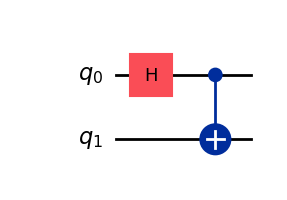
\includegraphics[width=0.5\textwidth]{Images/bell-states.png}
    \caption{Circuit for creating Bell States}
    \label{fig:bell-states}
\end{figure}
For example, suppose we wish to apply the circuit on state $\ket{01}$. Then the state after applying the
operation $H \otimes I$ will be $\frac{\ket{0}+\ket{1}}{\sqrt{2}}\otimes\ket{1}=\frac{\ket{01}+\ket{11}}{\sqrt{2}}$, and the state after applying the operation $CX$ will be $\frac{\ket{01}+\ket{10}}{\sqrt{2}}=\beta_{01}$. Similarly, we can create all the other Bell states. \textbf{Note that the Bell states $\ket{\Phi^{\pm}}=\frac{1}{\sqrt{2}}(\ket{00} \pm \ket{11}); \ket{\Psi^{\pm}}=\frac{1}{\sqrt{2}}(\ket{01} \pm \ket{10})$ form an orthonormal basis for $\mathbb{C}^4$.}

\begin{example}
    Given the state $\ket{\psi}=\frac{\ket{01}-\ket{10}}{\sqrt{2}}$, find whether the state is entangled or not.
    We prove this by contradiction, Assume that $\ket{\psi}$ can be written separately as $\alpha\ket{0}+\beta\ket{1} \otimes \gamma\ket{0}+\delta\ket{1}$.
    Thus, we get, 
    \begin{align*}
        \frac{\ket{01}-\ket{10}}{\sqrt{2}}&=\alpha\ket{0}+\beta\ket{1} \otimes \gamma\ket{0}+\delta\ket{1}\\
        &=\alpha\gamma\ket{00}+\alpha\delta\ket{01}+\beta\gamma\ket{10}+\beta\delta\ket{11}\\
    \end{align*}
    Comparing the equations we have, 
    \begin{align*}
        \alpha\gamma&=0 \\
        \alpha\delta&=\frac{1}{\sqrt{2}} \\
        \beta\gamma&=-\frac{1}{\sqrt{2}} \\
        \beta\delta&=0 \\
    \end{align*}
    No solution exists for the above equations, thus the given state is entangled as it cannot be written as a tensor product of two states.
\end{example}
Entanglement has applications in Teleportation and Superdense Coding which will be discussed next.
To get back the original input state from the Bell states we can use the following Circuit.
\begin{figure}[ht]
    \centering
    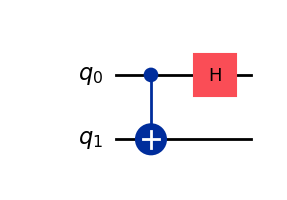
\includegraphics[width=0.5\textwidth]{Images/bell-states-rev.png}
    \caption{Circuit for Reversing Bell States}
    \label{fig:bell-states-rev}
\end{figure}
Here, we have used a reverse CNOT gate i.e. inverse of CNOT gate which is the CNOT gate since it's a self-inverse gate (Hermitian and Unitary).
Then we use the reverse Hadamard gate which is Hadamard Gate on the first qubit and the circuit will give back the original input state. (Hadmard gate is also self-inverse).
\begin{example}
    Verify that the Bell basis forms an orthonormal basis for the two qubit state space.

    We know that
    \[
    \ket{\beta_{xy}}=\frac{\ket{0y}+(-1)^x \ket{1\overline{y}}}{\sqrt{2}}
    \]
    where $x,y \in \{0,1\}$. Taking inner product with another bell state, we get,
    \begin{align*}
    \braket{\alpha_{pq}|\beta_{xy}}&=\left(\frac{\bra{0q}+(-1)^p\bra{1\overline{q}}}{\sqrt{2}}\right)\left(\frac{\ket{0y}+(-1)^x\ket{1\overline{y}}}{\sqrt{2}}\right)\\
    &=\frac{\braket{0q|0y}+(-1)^x\braket{0q|1\overline{y}}+(-1)^p\braket{1\overline{q}|0y}+(-1)^{x+p}\braket{1\overline{q}|1\overline{y}}}{2}
    \end{align*}
    Let $p=x$ and $q=y$, the above equation simplifies to, using the fact that $\braket{0q|0y}=\braket{1\overline{q}|q\overline{y}}=1$, else, $\braket{0q|q\overline{y}}=\braket{1\overline{q}|0y}=0$, and using the fact that $x=p \implies x+p=even$, we get,
    \begin{align*}
    &=\frac{1+0+0+(-1)^{x+p}1}{2}\\
    &=1
    \end{align*}
    Consider either $x\neq p$ or $y\neq q$ or both. In all the possible combinations of these cases, we would get, the value as $0$. Hence, the bell states form an orthonormal basis for two qubit states.

    Recall, that we can write any vector $\ket{\psi}$ in the 2-qubit state space as:
    \[
    \ket{\psi}=\alpha\ket{00}+\beta\ket{01}+\gamma\ket{10}+\delta \ket{11}
    \]
    as:
    \[
    \left(\frac{\alpha+\delta}{\sqrt{2}}\right)\ket{\beta_{00}}+\left(\frac{\alpha-\delta}{\sqrt{2}}\right)\ket{\beta_{01}}+\left(\frac{\beta+\gamma}{\sqrt{2}}\right)\ket{\beta_{10}}+\left(\frac{\beta-\gamma}{\sqrt{2}}\right)\ket{\beta_{11}}
    \]
    hence, this shows that the Belll states form a basis.
\end{example}
\section{No Cloning Theorem}
One of the counter-intuitive consequences of the laws of Quantum Mechanics is that 
it is impossible to create an exact copy of an arbitrary unknown quantum state. This is called the No Cloning Theorem.
More formally, 
\begin{theorem}
    Given an arbitrary unknown quantum state $\ket{\psi}$, it is impossible to create an exact copy of the state $\ket{\psi}$
    i.e. create the state $\ket{\psi}\ket{\psi}$. More precisely, it is impossible to start with two qubits in the state $\ket{\phi} \otimes \ket{0}$ and transform them to the state $\ket{\phi} \otimes \ket{\phi}$.
\end{theorem}
\begin{proof}
    From the Postulate 2: Evolution Postulate given in section \ref{subsection:Postulate 2}, from Axiom of Quantum Mechanics, for this to be possible there must be a Unitary transformation U such that $U\ket{\phi}\otimes \ket{0} = \ket{\phi}\otimes \ket{\phi}$. Thus, in order to prove that it is impossible to do so, it suffices to prove that no such unitary transformation exists. We start with proving that no such unitary transformation exists that can achieve this simultaneously for two states $\ket{\phi}=\alpha_0\ket{0}+\alpha_1\ket{1}$ and $\ket{\psi}=\beta_0\ket{0}+\beta_1\ket{1}$.

    Recall that a unitary transformation is a rotation of the Hilbert Space, and therefore necessarily preserves inner products. To be more precise, consider two quantum states: 
    \[
    \ket{\phi} \otimes \ket{0}= \alpha_0\ket{00}+\alpha_1\ket{10}
    \]
    and 
    \[\ket{\psi}\otimes \ket{0}=\beta_0\ket{00}+\beta_1\ket{10}
    \]
    Then, the inner product between them is given by 
    \[
    \braket{\phi0|\psi0}=\alpha^*_0\beta_0+\alpha^*_1\beta_1=\braket{\phi|\psi}
    \]
    Now consider the quantum states, 
    \begin{align*}
    \ket{\phi} \otimes \ket{\phi}&=(\alpha_0\ket{0}+\alpha_1\ket{1})\otimes (\alpha_0\ket{0}+\alpha_1\ket{1})\\
    &=\alpha^2_0\ket{00}+\alpha_0\alpha_1\ket{01}+\alpha_1\alpha_0\ket{10}+\alpha^2_1\ket{11}
    \end{align*}
    and
    \begin{align*}
    \ket{\psi}\otimes \ket{\psi}&=(\beta_0\ket{0}+\beta_1\ket{1})\otimes (\beta_0\ket{0}+\beta_1\ket{1})\\
    &=\beta^2_0\ket{00}+\beta_0\beta_1\ket{01}+\beta_1\beta_0\ket{10}+\beta^2_1\ket{11}
    \end{align*}
    Their inner product is 
    \begin{align*}
    \braket{\phi\phi|\psi\psi}&=(\bra{00}\alpha^{*2}_0+\bra{01}\alpha^*_0\alpha^*_1+\bra{10}\alpha^*_1\alpha^*_0+\bra{11}\alpha^{*2}_1)(\beta^2_0\ket{00}+\beta_0\beta_1\ket{01}+\beta_1\beta_0\ket{10}+\beta^2_1\ket{11})\\
    &=\alpha^{*2}_0\beta^2_0+\alpha^*_0\alpha^*_1\beta_0\beta_1+\alpha^*_1\alpha_0\beta_1\beta_0+\beta^2_0\beta^2_1\\
    &=(\alpha^*_0\beta_0+\alpha^*_1\beta_1)^2
    \end{align*}

    Now let us assume that we have a Unitary operator U and the two arbitrary quantum states $\ket{\phi}$ and $\ket{\psi}$ such that the action of U is defined as follows:
    \[
    \ket{\phi}\otimes \ket{0} \xrightarrow{U} \ket{\phi}\otimes \ket{\phi}
    \]
    \[
    \ket{\psi}\otimes \ket{0} \xrightarrow{U}\ket{\psi}\otimes \ket{\psi}
    \]
    Thus, clearly operator U corresponds to an operator which performs copying arbitrary quantum states.
    Since we are performing the same unitary transformation on both the states $\ket{\phi}$ and $\ket{\psi}$, thus the inner product before and after transformation must be the same, as a Unitary transformation corresponds to rotations in the complex Hilbert space. Their inner product before transformation is 
    \[
    \braket{\phi0|\psi0}=\alpha^*_0\beta_0+\alpha^*_1\beta_1
    \]
    Their inner product after the transformation will be:
    \[
    \braket{\phi\phi|\psi\psi}=(\alpha^*_0\beta_0+\alpha^*_1\beta_1)^2=\braket{\phi0|\psi0}^2=\braket{\phi|\psi}^2
    \]
    Thus, before transformation we had the inner product as $\braket{\phi|psi}$ and after the transformation we have the inner product as $\braket{\phi|\psi}^2$. Thus, in general, $\braket{\phi|\psi}\neq \braket{\phi|\psi}^2$ (It is equal only in the case when $\braket{\phi|\psi}=0$ or $1$ i.e. both the quantum states are orthonormal). Since, this is not true for any two arbitrary quantum states, thus our assumption that such a Unitary transformation U exists is wrong. Thus, by contradiction, we have proved that such a Unitary transformation U does not exists, hence, it is impossible to copy an arbitrary unknown quantum state $\ket{\phi}$ or in other words, to be more precise, no such unitary transformation $U$ exists which can perform the following transformation of $\ket{\phi} \otimes \ket{0} \rightarrow \ket{\phi} \otimes \ket{\phi}$.
\end{proof}
\begin{example}
    Explain how a device which, upon input of one of two non-orthogonal states $\ket{\psi}$ or $\ket{\varphi}$ correctly identified the state, could be used to build a device which cloned the states $\ket{\psi}$ and $\ket{\varphi}$, in violation of the no-cloning theorem. Conversely, explain how a device which cloned the states $\ket{\psi}$ and $\ket{\varphi}$, in violation of the no-cloning theorem. Conversely, explain how a device for cloning could be used to distinguish non-orthogonal quantum states.

    Given access to a device which can distinguish non-orthogonal states $\ket{\psi},\ket{\varphi}$ (without measurement), we can then design a quantum circuit that would map $\ket{\psi}\rightarrow \ket{\varphi}$ (or vice versa), allowing us to clone the states we like.

    Conversely, given a cloning device, we could clone $\ket{\psi}$ and $\ket{\varphi}$ an arbitrary number of times. Then, performing repeated measurements of the two states based on the measurement statistics in different measurement bases, we would (given enough measurements) be able to distinguish the two states based on the measurement statistics (there will of course be some error $\epsilon$ based on probabilistic considerations, but given that we have access to as many measurements of the states as we like, we are able to make this error arbitrarily low).
\end{example}




\section{Applications of Entanglement}
\subsection{Quantum Teleportation}
Suppose Alice has a qubit that she want to send to Bob. Let us say that the state of the qubit is $\alpha\ket{0}+\beta\ket{1}$. How many classical bits would be required to accomplish this task?

There are two reasonable answers to the question. the first answer is that the number of classical bits depends on the desired precision: $\alpha$ and $\beta$ are arbitrary complex numbers (with $|\alpha|^2 +|\beta|^2=1$), but Alice could send approximations of $\alpha$ and $\beta$ to Bob. The amplitudes $\alpha$ and $\beta$ cold require an infinite number of bits of precision to write them down exactly.

The second answer is that no number of classical bits of communication will suffice. Alice may not know $\alpha$ and $\beta$, and there is no way for her to perform measurements on her qubit that would reveal these numbers. Thus, she could not communicate this information to Bob because she could not even determine it for herself. There is also the possibility that Alice's qubit is entangled with one or more qubits (in which case of course we would not be able to describe the state of the qubit as $\alpha\ket{0}=\beta\ket{1}$). Classical communication from Alice to bob would not be able to somehow transmit this entanglement.

However, if we give Alice and Bob the additional resource of sharing a pair of qubits from bell states, then it becomes possible for Alice to transmit a qubit to Bob using classical communication by means of quantum teleportation. Specifically, two bits of classical information will be needed to perform this task (two classical bits need to be told to Bob). Depending upon which of four outcomes Alice announces to him, Bob performs one of four operations on his qubit, and voila, his qubit is in the required state.

Note that this doesn't violate the no cloning theorem because Alice's qubit was destroyed by measurement protocol before Bob created his copy.

They get together and create a Bell state $\beta_{00}$ and then 
distribute the quantum system. One qubit stays with Alice (say $\ket{\beta_A}$) 
and the other qubit goes to Bob (say $\ket{\beta_B}$).
Now Bob moves 100,000 light years away. Alice wishes to send Bob an Arbitrary state $\ket{\psi}$ to Bob.\\
\\
The teleportation protocol is as follows:
\begin{enumerate}
    \item Alice and Bob create a Bell state $\beta_{00}$. It is as shown in the figure \ref{fig:teleportation1} which has both the inputs $q_0=\ket{0}$ and $q_1=\ket{0}$.
    \begin{figure}[ht]
        \centering
        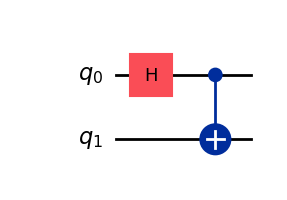
\includegraphics[width=0.5\textwidth]{Images/teleportation1.png}
        \caption{Creating Bell States}
        \label{fig:teleportation1}
    \end{figure}
    The state of the circuit after applying this state is the Bell state which is given as $\beta_{00}=\frac{\ket{00}+\ket{11}}{\sqrt{2}}$.
    Now, say the outcome of the first bit be $\ket{\beta_A}$ which is the state of the first qubit goes to Alice and the outcome of the second bit be $\ket{\beta_B}$ which is the state of the second qubit which goes to Bob.
    \item Alice applies a CNOT gate with the input state $\ket{\psi}$ as the control qubit and the state $\ket{\beta_A}$ as the target qubit. Then Alice applies a Hadamard gate on the input state $\ket{\psi}$. This is as shown in the figure \ref{fig:teleportation2} with $q_0=\ket{\psi}$ and $q_1=\ket{\beta_A}$.
    \begin{figure}
        \centering
        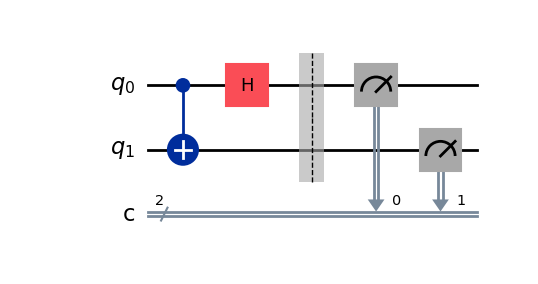
\includegraphics[width=0.75\textwidth]{Images/teleportation2.png}
        \caption{Alice's Operations}
        \label{fig:teleportation2}
    \end{figure}
    Thus the state here, is $\ket{\psi}\ket{\beta_{00}}$. Let the state $\ket{\psi}=\alpha\ket{0}+\beta\ket{1}$.
    Thus, 
    \[
        \ket{\psi}\ket{\beta_{00}}=(\alpha\ket{0}+\beta\ket{1})\otimes \frac{\ket{00}+\ket{11}}{\sqrt{2}}=\frac{\alpha\ket{000}+\alpha\ket{011}+\beta\ket{100}+\beta\ket{111}}{\sqrt{2}}
    \]
    Now applying $CNOT \otimes I$ with first bit as control bit and the second bit as the target bit and no operation on the third bit ($\ket{\beta_B}$ which is with Bob), we get,
    \[
        \frac{\alpha\ket{000}+\alpha\ket{011}+\beta\ket{110}+\beta\ket{101}}{\sqrt{2}}
    \]
    Now, applying Hadamard gate on the first bit, $(H\otimes I\otimes I)$, we get,
    \[
        \frac{\alpha\ket{000}+\alpha\ket{100}+\alpha\ket{011}+\alpha\ket{111}+\beta\ket{010}-\beta\ket{110}+\beta\ket{001}-\beta\ket{101}}{2}
    \]
    We further simplify this by factorizing only the first two qubits, we get,
    \[
        \frac{1}{2}\left[\ket{00}(\alpha\ket{0}+\beta\ket{1})+\ket{01}(\alpha\ket{1}+\beta\ket{0})+\ket{10}(\alpha\ket{0}-\beta\ket{1})+\ket{11}(\alpha\ket{1}-\beta\ket{0})\right]
    \]
    Now Alice does measurement of the first two qubits. Recall that the qubit $\ket{\psi}$ is already normalized i.e. $|\alpha|^2+|\beta|^2=1$. The probability of the first two qubits being $\ket{00}$ is $|\frac{\alpha}{2}|^2+|\frac{\beta}{2}|^2=\frac{|\alpha|^2+|\beta|^2}{4}=\frac{1}{4}$, similarly, 
    the probability of the first two qubits being $\ket{10}$ is $\frac{1}{4}$, the probability of the first two qubits being $\ket{01}$ is $\frac{1}{4}$ and the probability of the first two qubits being $\ket{11}$ is $\frac{1}{4}$.

    Note that there have been no measurements or communication at this point. Bob's qubit seems to depend on $\alpha$ and $\beta$, but this is not really so. There would be no way for Bob to transform and measure his qubit alone at this point so that he would learn anything about $\alpha$ and $\beta$. The state above has been expressed in a convenient way to determine the distribution of measurement outcomes and the resulting state of Bob's qubit after the measurements.
    Suppose upon measuring in the computational basis the two qubits by Alice they collapsed to $\ket{00}$, then the state of the system will be:
    \[
        \alpha\ket{000}+\beta\ket{001}=\ket{00}\otimes (\alpha\ket{0}+\beta{\ket{1}})
    \]
    Suppose upon measuring the two qubits by Alice they collapsed to $\ket{10}$, then the state of the system will be:
    \[
        \alpha\ket{100}-\beta\ket{101}=\ket{10}\otimes (\alpha\ket{0}-\beta\ket{1})
    \]
    Suppose upon measuring the two qubits by Alice they collapsed to $\ket{01}$, then the state of the system will be:
    \[
        \alpha\ket{011}+\beta\ket{010}=\ket{01}\otimes (\alpha\ket{1}+\beta\ket{0})
    \]
    Suppose upon measuring the two qubits by Alice they collapsed to $\ket{11}$, then the state of the system will be:
    \[
        \alpha\ket{111}-\beta\ket{110}=\ket{11}\otimes (\alpha\ket{1}-\beta\ket{0})
    \]
    All of the above are possible with a probability of $\frac{1}{4}$. 
    \item Now Alice sends the result of the measurement to Bob. Bob applies the necessary operations to get the original state $\ket{\psi}=\alpha\ket{0}+\beta\ket{1}$.
    
    \begin{itemize}
        \item Suppose Alice measured the first two qubits to be $\ket{00}$, then Bob applies no operation.
        \[
            \alpha\ket{000}+\beta\ket{001}=\ket{00}\otimes (\alpha\ket{0}+\beta\ket{1})
        \]
        \item Suppose Alice measured the first two qubits to be $\ket{10}$, then Bob applies the Z gate on his qubit to get the original state.
        \[ 
            (I\otimes I \otimes Z)(\alpha\ket{100}-\beta\ket{101})=\alpha\ket{100}+\beta\ket{101}=\ket{10}\otimes (\alpha\ket{0}+\beta\ket{1})
        \]
        \item Suppose Alice measured the first two qubits to be $\ket{01}$, then Bob applies the X gate on his qubit to get the original state.
        \[ 
            (I\otimes I\otimes X)(\alpha\ket{011}+\beta\ket{010})=\alpha\ket{010}+\beta\ket{011}=\ket{01}\otimes (\alpha\ket{0}+\beta\ket{1})
        \]
        \item Suppose Alice measured the first two qubits to be $\ket{11}$, then Bob applies the X and Z gate on his qubit to get the original state.
        \[ 
          (I\otimes I\otimes ZX)(\alpha\ket{111}-\beta\ket{110}))=\alpha\ket{110}+\beta\ket{111}=\ket{11}\otimes (\alpha\ket{0}+\beta\ket{1})
        \]
    \end{itemize}
    Thus, we have teleport ed the unknown state $\ket{\psi}$ from Alice to Bob. Note that during this protocol, the Bell state of the qubits is destroyed upon measurement by Alice and thus, cannot be done again. Note that in the figure \ref{fig:teleportation} circuit diagram we see that the measurement results in a classical bits and the gates then act on one classical bit and one qubit. generally we will only do this when the classical bit is a control bit for some operation. all that this means is that if the (classical) control bit is 1 then perform the corresponding operation on the qubit ($\sigma_Z$ or $\sigma_X$), otherwise do nothing.
\end{enumerate}
To summarise, we start with the following scenario. Alice and Bob share two qubits in the state $a\ket{00}+b\ket{11}$. Alice and Bob don't know the amplitudes $a$ and $b$. how can Bob end up with the state $a\ket{0}+b\ket{1}$? An easy way to achieve this is to perform a CNOT gate on the two qubits with Bob's qubit as the control, and Alice's qubit as the target. But this requires an exchange of quantum information. What if Alice and Bob can only exchange classical information?

    The way is Alice performs a hadamard on her qubit. The state of the two qubits is now $a/\sqrt{2}(\ket{0}+\ket{1})\ket{0}+b/\sqrt{2}(\ket{0}-\ket{1})\ket{1}=1/\sqrt{2}\ket{0}(a\ket{0}+b\ket{1})+1/\sqrt{2}\ket{1}(a\ket{1}-b\ket{1})$. Now if Alice measures her qubit in the standard basis, if the measurement outcome is 0, the Bob's qubit is desired $a\ket{0}+b\ket{1}$. If the measurement outcomes is $1$, then Bob's qubit is $a\ket{0}-b\ket{1}$. But in this case if Bob were to apply a phase flip gate (Z) to his qubit, it would end up in the desired state $a\ket{0}+b\ket{1}$,
    
    Back to Teleportation. Alice has a qubit in the state $a\ket{0}=b\ket{1}$, and Alice and Bob share a Bell state. Is there a way for them to convert their joint state to $a\ket{00}+b\ket{11}$, without exchanging any quantum information? If they succeed, then by our previous discussion Alice can teleport her qubit to Bob. Consider what happens if Alice applies a CNOT gate with her qubit $a\ket{0}+b\ket{1}$ as the control qubit, and her share of the Bell state as the target qubit.
    \[
    \ket{\phi} \otimes \ket{\psi} = \sum_{i=0,1} a_i\ket{i} \otimes \sum_{j=0,1} \frac{1}{\sqrt{2}} \ket{j,j}
    \]
    After passing through the CNOT gate this becomes
    \[
    \sum_{i,j} a_i\ket{i,i \oplus l}
    \]
    Now A measures the middle qubit. Suppose it is measured as $l$; then $l=i\oplus j \implies j=i\oplus l$. The state is now
    \[
    \sum_i a_i\ket{i,i\oplus l}
    \]
    next, A transmits $L$ to $B$. If $l=0$, $B$ takes no action, while if $l=1$, then $B$ performs a bit flip $X$, on his qubit, resulting in the desired state
    \[
    \sum_i a_i\ket{i,i}
    \]
    We already saw how to teleport once we achieved this state. Putting it all together, the following quantum circuit \ref{fig:teleportation} circuit describes the resulting teleportation protocol. The topmost qubit is the unknown qubit that Alice wishes to teleport, the second and third qubits are initially in a Bell state. The measurement of the middle qubit after performing the CNOT gate sets up the state $\sum_j a_j\ket{j,j}$ on the first and third qubit. Moreover, $A'$ application of the Hadamard gate on the first qubit induces the transformation
    \[
    \sum_j a_j\ket{j,j} \rightarrow \sum_{ij} a_j (-1)^{ij} \ket{i,j}
    \]
    Finally A measures $i$ and sends the measurement to $B$. The state is now:
    \[
    \sum_j a_j (-1)^{ij} \ket{j}
    \]
    If $i=0$ then we are done; if $i=1$ then $B$ applies a phase flip. In either case the state is now $a_0\ket{0}+a_1\ket{1}$. So A has transported the quantum state to B simply by sending two classical bits.
The final Teleportation circuit is as shown in the figure \ref{fig:teleportation}.
\begin{figure}
    \centering
    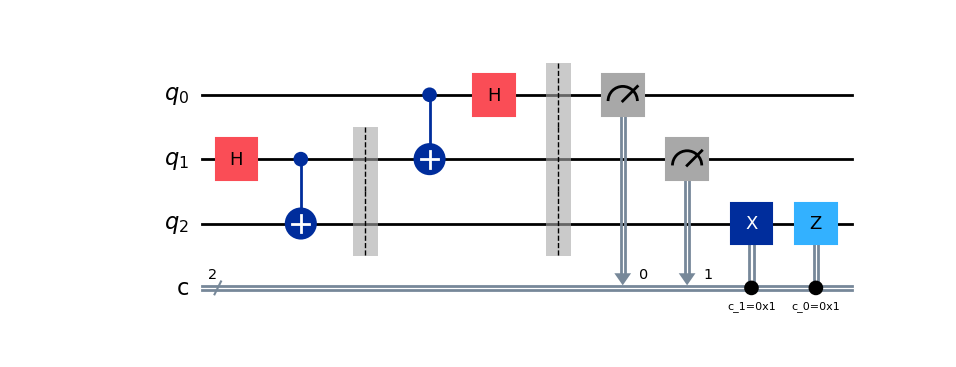
\includegraphics[width=1\textwidth]{Images/teleportation.png}
    \caption{Teleportation Circuit}
    \label{fig:teleportation}
\end{figure}
We can see from the figure that the measurement output from the Alice's qubits act as control bits for applying Z and X gate.
If the first qubit is 1 then we apply the Z gate, if the second qubit is 1 then we apply the X gate. Based on the Alice's output we can decide whether to apply  Thus the circuit shown in the figure \ref{fig:teleportation}, show that
after Alice's measurement the bits act as control bits for the operations to be applied by Bob.


Something stronger is actually true. If Alice's initial qubit was entangled with other qubits, this entanglement will be preserved. In other words, teleportation works like a perfect quantum channel - it is exactly as if Alice had physically sent her qubit to Bob. \textbf{If Alice's qubit had been entangled with some other qubits, then teleportation preserves this entanglement: Bob then receives a qubit that is entangled in the same way as Alice's original qubit was. Note that qubit on Alice's side has been destroyed: teleporting moves a qubit from Alice to Bob, rather than copying it.}

\subsection{Superdense Coding}
Suppose Alice and Bob are connected by a quantum communications channel. By this we mean, for example, that they cannot communicate qubits over an optical fibre using polarized photons. Is this, much more powerful than a classical communication channel, over which only classical bits may be transmitted? The answer seems obvious, since a classical bit is a special case of quantum bit. And a qubit appears to encode an infinite number of bits of information, since to specify this state we must specify two complex numbers. However, the truth is a little more subtle, since the axioms of quantum mechanics also restrict how we may access information about the quantum state by measurement. So the question is ``how many classical bits can Alice transmit to Bob in a message consisting of a single qubit?". We will show that if Alice and Bob share entanglement in the form of a Bell state, then Alice can transmit two classical bits by transmitting just one qubit over the quantum channel. 

The overall idea is this: say Alice and Bob share $\ket{\Phi^{+}}=\frac{1}{\sqrt{2}}(\ket{00}+\ket{11})$. Alice can transform this shared state to any of the four Bell basis state $\ket{\Phi^{+}},\ket{\Phi^{-}},\ket{\Psi^{+}},\ket{\Phi^{-}}$ by applying a suitable quantum gate just to her qubit. now if she transmits her qubit to bob, he holds both qubit of a bell basis state and can perform a measurement in the Bell basis to distinguish which of the four states he holds.

Let's now see the details of Alice's protocol: if Alice wishes to transmit the two bit messages $b_1b_2$, she applies a bit flip X to her qubit if $b_1=1$ and a phase flip $Z$ to her qubit if $b_2=1$. you should verify that in the four cases $00,01,10,11$ this results in the two being in the state $\ket{\Phi^{+}},\ket{\Phi^{-}},\ket{\Psi^{+}},\ket{\Psi^{-}}$ respectively.

After receiving Alice's qubit, Bob measures the two qubits in the bell basis by running the circuit shown in figure \ref{fig:superdense3} $((H\otimes I) \cdot CNOT)$, then measuring in the standard basis.

Note that Alice did really use the two qubits total to transmit the two classical bits. After all, Alice and Bob somehow had to start with a shared Bell State. However, the first qubit - Bob's half of the bell state - could have been sent well before Alice had decided what message she wished to send to Bob. It is natural to view entanglement as a resource as we will see; and when Alice and Bob each have a qubit and the two of them are in the state above, it is natural to imagine that Alice and Bob share one unit (i.e.e one entangled bit, or e-bit for short) of entanglement. Given the additional resource of a shared e-bit of entanglement, Alice will be able to transmit both classical bits to Bob by sending just one qubit.

One can show that it is not possible to do any better. No more than two classical bits can be transmitted by sending just one qubit.

In Super dense coding we can send two classical bits from one place to another but using only one qubit. 
Alice and Bob create a bell state $\beta_{00}$ and then distribute the qubits. Alice takes the first qubit and Bob takes the second qubit.
Bob now moves light years away. Alice now wishes to send two classical bits to Bob. The protocol is as follows:
\begin{enumerate}
    \item \textbf{Preparing Bell States: }Alice and Bob create a Bell state $\beta_{00}$.
    The state of the circuit after applying this state is the Bell state which is given as $\beta_{00}=\frac{\ket{00}+\ket{11}}{\sqrt{2}}$.
    Now, say the first bit be $\ket{\beta_A}$ which is the qubit that goes to Alice and the second bit be $\ket{\beta_B}$ which is the qubit which goes to Bob.
    \begin{figure}[ht]
        \centering
        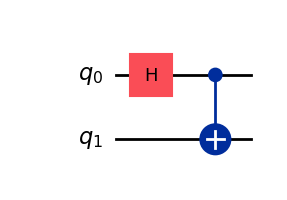
\includegraphics[width=0.5\textwidth]{Images/superdense-coding1.png}
        \caption{Creating Bell States}
        \label{fig:superdense1}
    \end{figure}
    This is how the Bell state is created shown in the figure \ref{fig:superdense1}.
    \item \textbf{Alice Encoding: } Alice applies the necessary operations to send the two classical bits to Bob.
    These operations are done on the first qubit which is with Alice as follows in the figure \ref{fig:superdense2}.
    \begin{figure}[ht]
        \centering
        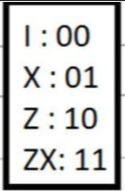
\includegraphics[width=0.1\textwidth]{Images/superdense-coding2.png}
        \caption{Alice's Encoding}
        \label{fig:superdense2}
    \end{figure}
    \begin{itemize}
        \item If Alice wishes to send $00$, then she applies no operation.
        \[
            (I\otimes I)\frac{\ket{00}+\ket{11}}{\sqrt{2}}=\frac{\ket{00}+\ket{11}}{\sqrt{2}}
        \]
        \item If Alice wishes to send $01$, then she applies the Pauli - X gate on her portion of Bell state.
        \[
            (X\otimes I)\left(\frac{\ket{00}+\ket{11}}{\sqrt{2}}\right)=\frac{\ket{10}+\ket{01}}{\sqrt{2}}
        \]
        \item If Alice wishes to send $10$, then she applies the Pauli-Z gate on the qubit.
        \[
            (Z \otimes I)\left(\frac{\ket{00}+\ket{11}}{\sqrt{2}}\right)=\frac{\ket{00}-\ket{11}}{\sqrt{2}}
        \]
        \item If Alice wishes to send $11$, then she applies the Pauli-X and Pauli-Z gate on the qubit.
        \[
            (XZ \otimes I)\left(\frac{\ket{00}+\ket{11}}{\sqrt{2}}\right)=\frac{\ket{10}-\ket{01}}{\sqrt{2}}
        \]
    \end{itemize}
    In summary, in order to send the two classical bits $b_1b_2$, Alice applies Z first if $b_1=1$ (if $b_1=0$ he does not apply Z, he applies I i.e. does nothing) and then applies X it $b_2=1$ (if $b_2=0$ he does not apply X, he applies I i.e. does nothing).
    \item \textbf{Bob Decoding: }Now Alice sends her portion of Bell state qubit to Bob. Bob then applies the necessary operations to get the two classical bits.
    Bob performs the following operations on the qubit he received from Alice:
    He applies CNOT gate with the first qubit (Qubit sent by Alice) as the control qubit and the second qubit (his qubit) as the target qubit. Then he applies Hadamard gate on the first qubit (Qubit sent by Alice).
    Then she performs the measurement. The measurement will give the two classical bits that Alice wished to send.
    This circuit for this is as shown in the figure \ref{fig:superdense3}.
    \begin{figure}[ht]
        \centering
        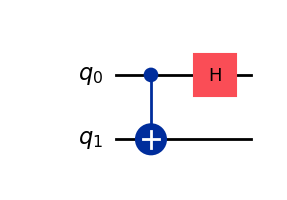
\includegraphics[width=0.5\textwidth]{Images/superdense-coding3.png}
        \caption{Bob's Decoding}
        \label{fig:superdense3}
    \end{figure}
    \begin{itemize}
        \item If Alice wished to send $00$, then the state of the system is currently $\frac{\ket{00}+\ket{11}}{\sqrt{2}}$. Thus, after applying the CNOT gate,
        \[
            CNOT\left(\frac{\ket{00}+\ket{11}}{\sqrt{2}}\right)=\frac{\ket{00}+\ket{10}}{\sqrt{2}}
        \]
        Now, after applying the Hadamard Gate on the first qubit we get,
        \[
            (H \otimes I)\left(\frac{\ket{00}+\ket{10}}{\sqrt{2}}\right)=\frac{\ket{00}+\ket{10}+\ket{00}-\ket{10}}{2}=\ket{00}
        \]
        Thus, on measurement, the two classical bits are $00$.
        \item If Alice wished to send $01$, then the state of the system is currently $\frac{\ket{10}+\ket{01}}{\sqrt{2}}$. Thus, after applying the CNOT gate,
        \[
            CNOT\left(\frac{\ket{10}+\ket{01}}{\sqrt{2}}\right)=\frac{\ket{11}+\ket{01}}{\sqrt{2}}
        \]
        Now, after applying the Hadamard Gate on the first qubit we get,
        \[
            (H\otimes I)\left(\frac{\ket{11}+\ket{01}}{\sqrt{2}}\right)=\frac{\ket{01}-\ket{11}+\ket{01}+\ket{11}}{2}=\ket{01}
        \]
        \item If Alice wished to send $10$, then the state of the system is currently $\frac{\ket{00}-\ket{11}}{\sqrt{2}}$. Thus, after applying the CNOT gate,
        \[
            CNOT\left(\frac{\ket{00}-\ket{11}}{\sqrt{2}}\right)=\frac{\ket{00}-\ket{10}}{\sqrt{2}}
        \]
        Now, after applying the Hadamard Gate on the first qubit we get,
        \[
            (H\otimes I)\left(\frac{\ket{00}-\ket{10}}{\sqrt{2}}\right)=\frac{\ket{00}+\ket{10}-\ket{00}+\ket{10}}{2}=\ket{10}
        \]
        \item If Alice wished to send $11$, then the state of the system is currently $\frac{\ket{10}-\ket{01}}{\sqrt{2}}$. Thus, after applying the CNOT gate,
        \[
            CNOT\left(\frac{\ket{10}-\ket{01}}{\sqrt{2}}\right)=\frac{\ket{11}-\ket{01}}{\sqrt{2}}
        \]
        Now, after applying the Hadamard Gate on the first qubit we get,
        \[
            (H\otimes I)\left(\frac{\ket{11}-\ket{01}}{\sqrt{2}}\right)=\frac{\ket{01}-\ket{11}-\ket{01}-\ket{11}}{2}=-\ket{11}
        \]
        Thus, upon measurement the two classical bits are $11$.
    \end{itemize}
    When Bob measures at the end of the protocol, it is clear that he sees $b_1b_2$ with certainty.
\end{enumerate}

The final Superdense coding circuit is as shown in the figure \ref{fig:superdense-coding}.
% Add four subfigures
\begin{figure}[ht]
    \centering
    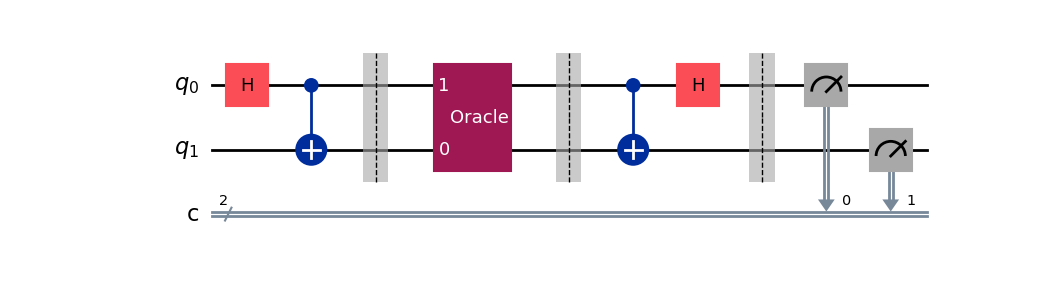
\includegraphics[width=1\textwidth]{Images/superdense-coding4.png}
    \caption{Superdense Coding Circuit}
    \label{fig:superdense-coding}
\end{figure}
\begin{example}
    Suppose $E$ is any positive oeprator acting on Alice's qubit. Show that $\braket{\psi|E\otimes I|\psi}$ takes the same value when $\ket{\psi}$ is any of the four Bell states. Suppose some malovelent third party ('Eve') intercepts Alice's qubit on the way to Bob in the superdense coding protocol. Can eve infer anything about which of the four possible bit strings $00,01,10,11$ Alice is trying to send? If so how, or if not, why not?

    Since E is a positive operator ($\implies E=E^{\dagger} \quad \text{and} \quad \bra{x}E\ket{x}\geq 0 \quad \forall x$), it is a hermitian matrix (an obseravable) with all real eigen values greater than 0. Thus, E is a measurement operator.
        We can write the above expression as,
        \begin{align*}
        \bra{\beta}_{xy}(E\otimes I)\ket{\beta}_{xy}&=\frac{1}{2}\left(\bra{0y}+(-1)^x\bra{1\overline{y}}\right)(E\otimes I)\left(\ket{0y}+(-1)^x\ket{1\overline{y}}\right)\\
        &=\frac{1}{2}\left(\bra{0}E\ket{0} \otimes \braket{y} + (-1)^x \bra{0}E\ket{1} \otimes \bra{y}\ket{\overline{y}} \right)\\
        & \quad + \frac{1}{2}\left((-1)^x\bra{1}E\ket{0} \otimes \bra{\overline{y}}\ket{y} + (-1)^{2x}\bra{1}E\ket{1} \otimes \bra{\overline{y}}\ket{\overline{y}} \right)
        \end{align*}
        Now since $ y \in \{0,1\}$ and the state $\ket{y}$ is unit norm, we can write $\braket{y}=1$ and $\bra{y}\ket{\overline{y}}=\bra{\overline{y}}\ket{y}=0$ (since $\ket{y}$ and $\ket{\overline{y}}$ will always be orthonormal states). Thus, on substituting this, the above expression simplifies to,
        \[
        \bra{\beta}_{xy}(E\otimes I)\ket{\beta}_{xy}=\frac{1}{2}\left(\bra{0}E\ket{0} + \bra{1}E\ket{1} \right)
        \]
        Thus, irrespective of the values of $x$ and $y$, the value of $\bra{\beta}_{xy}(E\otimes I)\ket{\beta}_{xy} = \bra{\psi}(E \otimes I)\ket{\psi}=\frac{1}{2}(\bra{0}E\ket{0}+\bra{1}E\ket{1})$ which is same for all the four bell states (as it does not depend on values of $x$ and $y$).
        Thus, for any positive operator (say $E$) acting on the first qubit of a 2-qubit bell state takes the same value irrespective of the bell state.
        \[
            \bra{\beta}_{xy}(E\otimes I)\ket{\beta}_{xy}=\left(\frac{\bra{0}E\ket{0} + \bra{1}E\ket{1} }{2}\right)
        \]
        In the superdense coding protocol recall that Alice sends its one qubit (which is in one of the Bell states) to Bob after performing the required operations based on what two classical bits Alice wishes to communicate to Bob. 
        While sending, if an unauthorized third party Eve intercepts Alice's qubit being sent to Bob across the channel then as can be seen from the result in (a), since Eve has only one qubit no matter what observable (hermitian operator) she uses to measure the Alice's qubit being sent, she would always get the same measurement outcome
        \[
        \bra{\psi}(E\otimes I)\ket{\psi}=\frac{1}{2}(\bra{0}E\ket{0}+\bra{1}E\ket{1})
        \]
        Since the probability of getting any of the eigen value of $E$ (say m) is same and after the measurement the state of the qubit will be in the 
        Eigen state corresponding to the eigen value m. Thus, no matter what operator Eve uses it will always outcome one of its eigen values with the same probability and the post-measurement state would be the eigen ket corresponding to the outcome (eigenvalue) of the measurement. Thus, Eve cannot infer anything about which of the four possible bit pairs 00, 01, 10, 11 Alice is trying to send.
\end{example}
\subsection{The CHSH Game}
The CHSH game is named after four people (Clauser, Horne, Shimony, and Holt) who in 1969 wrote a paper saying ``this is how to think about what Bell did". The game itself doesn't involve quantum mechanics, but quantum mechanics can help us win it. The CHSH game could be seen as a precursor to quantum computing, in that it's one of the first cases when people looked to see which information processing tasks quantum mechanics helps us solve better - and where they enforced a conceptual separation between the tasks itself (which is classical) and the strategy to solve it (which can be quantum).

The idea is that Alice and Bob are placed in separate rooms and are both given a challenge bit ($x$ and $y$ respectively) by a referee, Charlie. The challenge bits are chosen uniformly at random, and independently of each other. Alice sends an answer bit, $a$, back to the referee and Bob sends an answer bit $b$. Alice and Bob ``win" the game iff
\[
a+b=xy \quad(\text{mod 2})
\]
Alice and Bob are allowed to agree n a strategy in advance (in other words correlate their answers)( and to share random bits. A classical strategy to maximize winning probability is simply that Alice and Bob always send the referee $a=b=0$, regardless of what $x$ and $y$ are. In this case, Alice and Bob win $75\%$ of the time, losing only if $x$ and $y$ are both $1$. To prove that this is optimal the first step is to notice that, without loss of generality, Alice and Bob's strategy can be assumed to be deterministic (i.e., to involve no random bits besides $x$ and $y$ themselves). Any probabilistic strategy is equivalent to a mixture that does at least as well as the average, so we can derandomize the protocol without negatively impacting the overall success probability; this is called a convexity argument. This convexity argument holds true even if we assume Alice and Bob have access to shared randomness.

Let's treat Alice;s output bit $a$ as a function of her input bits $x$ and Bob's output bit $b$ as a function of his input bit $y$. In order to win the game they need to select bits $a$ and $b$ satisfying the equation
\[
a(x)+b(y)=xy \quad \text{(mod 2)}
\]
You can easily check by enumerating cases (using the winning conditions in Table~\ref{tab:chsh_win_lose}) that this equation can't possibly hold for al $4$ values of $x$ and $y$! At best it can hold for $3$ of the $4$ values of $x$ and $y$!, which is exactly what the trivial strategy above (always send back $0$) achieves.

The Bell inequality, in this framework, is just slightly boring statement we proved above. Namely, tha the maximum classical win probability in the CHSH game is $75\%$. bell noticed an additional fact, though. If Alice and Bob have access to a pre-shared Bell pair, $\frac{\ket{00}+\ket{11}}{\sqrt{2}}$, then there's a better strategy. In that case, in fact their maximum probability is 
\[
P=\cos^2\left(\frac{\pi}{8}\right)\approx 85\%
\]
How do they use entanglement to achieve an important over the classical win probability.

\subsection*{CHSH Game: Quantum Strategy}
In the previous lecture we talked about the CHSH Game, and how no classical strategy lets Alice and Bob win it more than $75\%$ of the time. In this lecture we'll see how, by using entanglement, they can win $\approx 85\%$ of the time, an delve deeper to try understand what's going on.

The quantum strategy for the CHSH game assumes that before Alice and Bob go to their separate rooms and receive their challenges they pre-share $1$-ebit of entanglement. In other word, Alice and Bob each share 1 half of a Bell pair, $\frac{\ket{00}+\ket{11}}{\sqrt{2}}$ Upon receiving their challenge bits from the referee, Charlie , Alice and Bob measure their respective qubits in different bases depending on whether their input bits $x$ and $y$ are $0$ or $1$. Based on the results of their measurements, Alice and Bob then output bits $a$ and $b$ based on the outcomes.

Before explicitly stating the protocol we'll first quickly introduce notation for four states which will play a crucial role in the protocol. These four states are
\[
\ket{\pi/8}=\cos\frac{\pi}{8}\ket{0} + \sin\frac{\pi}{8}\ket{1} ,\quad \ket{\frac{5\pi}{8}}=\cos
\left(\frac{5\pi}{8}\right) \ket{0}+\sin\left(\frac{5\pi}{8}\right)\ket{1}
\]
\[
\ket{-\pi/8}=\cos\left(-\frac{\pi}{8}\right)\ket{0}+\sin\left(-\frac{\pi}{8}\right)\ket{1},\quad \ket{\frac{3\pi}{8}}=\cos\left(\frac{3\pi}{8}\right) \ket{0}+\sin\left(\frac{3\pi}{8}\right) \ket{1}
\]
The states correspond to a rotation of the standard basis either $\pi/8$ radians counterclockwise or $\pi/8$ radians clockwise. We saw at least one of these states in a different context back when discussing the distinguish ability of quantum states - though we may not have written it explicitly in this form - and on the homework in calculating the optimal basis for distinguishing the $\ket{0}$ state from the $\ket{+}$ state. Recall that measuring in a basis $\{\ket{v},\ket{w}\}$ is equivalent to applying a unitary transformation into the standard basis followed by a measurement in the standard basis. As such, we can perform the measurements in the $\{\ket{\pi/8},\ket{5\pi/8}\}$ and $\{\ket{-\pi/8},\ket{3\pi/8}\}$ bases by applying unitary transformation (in this case $R_{\pi/8}$ and $R_{-\pi/8}$, respectively) followed by a measurement in the standard basis.

Alice and Bob's measurement strategy is as follows:
\begin{itemize}
    \item If $x=0$ then Alice measures in the $\{\ket{0},\ket{1}\}$ basis. If the outcome of Alice's measurement is $\ket{0}$, then she sends back $a=0$. If the oucome of Alice's measurmeent is $\ket{1}$, then she sends back $a=1$.
    \item If $x=1$ then Alice measures in the $\{\ket{+},\ket{-}\}$ basis. If the outcome of Alice's measurement is $\ket{+}$, then she sends back $a=0$. If the outcome of Alice's measurement is $\ket{-}$, then she sends back $a=1$.
    \item If $y=0$ then Bob measures in the $\{\ket{\pi/8},\ket{5\pi/8}\}$ basis. If the outcome of Bob's measurement is $\ket{\pi/8}\}$, thenhe sends back $b=0$;. If the outcome of Bob's measurement is $\ket{5\pi/8}$, then he sends back $b=1$.
    \item If $y=1$ then Bob measures in the $\{\ket{-\pi/8},\ket{3\pi/8}\}$ basis. If the outcome of Bob's measurement is $\ket{-\pi/8}$, then he sends back $b=0$, If the outcome of Bob's measurement is $\ket{3\pi/8}$, then he sends back $b=1$.
\end{itemize}
This strategy has the amazing property that Alice and Bob win with probability $\cos^2(\pi/8)$ for all possible values of $x$ and $y$.

\subsection*{Analysis of Protocol}
So why does the strategy work $85\%$ of the time?Let's analyze the results on a case-by-case basis. We can assume without loss of generality that Alice measures first, due to the No-Communication Theorem. The first case is where Alice gets $x=0$ and Bob gets $y=0$. As always, Alice and Bob will win if they return $a$ and $b$ such that $a+b=xy=0\quad \text{(mod 2)}$. Alice measures in the $\{\ket{0},\ket{1}\}$ basis and Bob measures in the $\{\ket{\pi/8},\ket{5\pi/8}\}$ basis. Suppose Alice see $\ket{0}$. Then the state of Bob's qubit also collapses to $\ket{0}$. When Bob measures his now collapsed qubit in the $\{\ket{\pi/8},\ket{5\pi/8}\}$ basis he sees either $\ket{\pi/8}$ or $\ket{5\pi/8}$ with probabilities
\[
P(\ket{\pi/8})=|\braket{0|\pi/8}|^2=|\cos(\pi/8)|^2=\cos^2\pi/8
\]
\[
P(\ket{5\pi/8})=|\braket{0|5\pi/8}|^2=|\cos(5\pi/8)|^2=|\sin(\pi/8)|^2=\sin^2\pi/8
\]
Now suppose Alice sees $\ket{1}$. Then Bob's qubit collapses to $\ket{1}$and when he measures in the $\{\ket{\pi/8},\ket{5\pi/8}\}$ basis he sees either $]ket{\pi/8}$ or $\ket{5\pi/8}$ with probabilities
\[
P(\ket{\pi/8})=|\braket{1|\pi/8}|^2=|\sin(\pi/8)|^2=\sin^2\left(\frac{\pi}{8}\right)
\]
\[
P(\ket{5\pi/8})=|\braket{1|5\pi/8}|^2=|\sin(5\pi/8)|^2=|\cos(\pi/8)|^2=\cos^2\left(\frac{5\pi}{8}\right)
\]
Recall that the goal is to output $a$ and $b$ such that $a+b=xy(\text{mod 2})$. In this first case $xy=0$ so Alice and Bob win if they return either $a=b=0$ or $a=b=1$. The probability they win is thus given by
\begin{align*}
&P(a=0)P(b=0|a=0)+P(a=1)P(b=1|a=1)\\
&=\frac{1}{2}\cos^2\left(\frac{\pi}{8}\right)+\frac{1}{2}\cos^2\left(\frac{\pi}{8}\right)\\
&=\cos^2\left(\frac{\pi}{8}\right)
\end{align*}
The analysis for the case where $x=0$ and $y=1$ and the case where $x=1$ and $y=0$ is very similar to the case above, so we'll leave it to the reader to verify that the protocol succeeds with probability $\cos^2(\pi/8)$ in those cases. Somewhat more interesting is the case where $x=y=1$. In order to analyze this case it is useful to note that the Bell state takes the same general form regardless of which basis we choose to write it in. In this case we'll choose to write it as $\frac{\ket{++}+\ket{--}}{\sqrt{2}}$. Therefore, when Alice measures in the $\{\ket{+},\ket{-}\}$ basis she sees both $\ket{+}$ and $\ket{-}$ with equal probability. in either case, Bob's qubit collapses to the same outcome. Suppose Alice sees $\ket{+}$ .then Bob measures his qubit in the $\{\ket{-\pi/8},\ket{3\pi/8}\}$ basis he sees $\ket{-\pi/8}$ with probability
\[
P(\ket{-\pi/8})=|\braket{+|-\pi/8}|^2=\sin^2\left(\frac{\pi}{8}\right)
\]
and he sees $\ket{3\pi/8}$ with probability
\[
P(\ket{3\pi/8})=1-P(\ket{-\pi/8})=1-\sin^2(\pi/8)=\cos^2\left(\frac{\pi}{8}\right)
\]
Likewise, when Alice sees $\ket{-}$, Bob sees either $\ket{-\pi/8}$ with probability
\[
P(\ket{-\pi/8})=|\braket{-|-\pi/8}|^2=\cos^2\left(\frac{\pi}{8}\right)
\]
The win condition for Alice and Bob when $x=y=1$ is for $a$ and $b$ to have odd parity. As such, the win probability is:
\begin{align*}
    &P(a=0)P(b=1|a=0)+P(a=1)P(b=0|a=1)\\
    &=\frac{1}{2}\cos^2\left(\frac{\pi}{8}\right)+\frac{1}{2}\cos^2\left(\frac{\pi}{8}\right)\\
    &=\cos^2\left(\frac{\pi}{8}\right)
\end{align*}
So to sum up, in all four cases the quantum protocol achieves a win probability of $\cos^2\left(\frac{\pi}{8}\right)\approx 85\%$, higher than the classical win probability of $75\%$.

\subsection*{CHSH game: Interpretations and Local Realism}
How does this game relate to hidden-variable theories? Well, if all correlations between the qubits could be explained by stories like ``if anyone asks, we're both 0", then we'd make a firm prediction that Alice and Bob can win the CHSH game with at most $75\%$ probability (because that's how well they can do by pre-sharing arbitrary amounts of classical randomness). This would be consisten with the principle of local realism, which we discussed before. So, if they play the game repeatedly and demonstrate that they can win more than $75\%$ of the time, then we must conclude local realism doesn't hold. Notice that nowhere in this argument did we need to presuppose that quantum mechanics is true.

Does Alice and Bob's ability to succeed more than $75\%$ of the time mean that they are communicating? Well, we know it's not possible for either to send a signal to the other using the entanglement by the No-communication theorem. One way to understand what's going on is to work out Alice and Bob's density matrices explicitly.

Bob's initial local density matrix is
\[
\begin{bmatrix}
    \frac{1}{2} & 0 \\
    0 & \frac{1}{2}
\end{bmatrix}
\]
and after Alice measures it's still
\[
\begin{bmatrix}
    \frac{1}{2} & 0 \\
    0 & \frac{1}{2}
\end{bmatrix}
\]
So in that sense, no signal has been communicated from Aclie to Bob. Nevertheless, if you knew both Alice's  measurement and its outcome, then you could update Bob's lcocal density matrix to that of a pure state. That shouldn't worry us even classically. even if you condition on what Alice sees then you can change your predictions for Bob.

Imagine a heirarcy of possibilities for what the universe allows. Classical Loacal Realism is at the bottom. here you only ever need to use classical probability theory when you have incomplete information about physical systems, and also signals propagate at most at the speed of light. at the top of the hierarchy is the Faster-Than-Light (FTL) Science-fiction Utopia, where Alice and Bob can communicate instantaneously, can travel faster than light. So when they read pop-science articles about how classical local realism doesn't hold, they think ``OK, then we must live in the FTL sci-fi utopia". Instead, the truth - according to quantum mechanics is somewhere in between these two, and the distinction is so subtle that perhaps no science-fiction write could ever have had imagination to invent it. We live in a world where there's no classical local realism, a purely classical simulation of our universe would have to include FTL communication, but our universe itself does not. Maybe no science function writer ever came up with the possibility simply because it's hard to think of a plot that requires Alice and Bob to win the CHSH game $85\%$ of the time instead of $75\%$!

Indeed, experimental violations of the Bell inequality are key piece of evidence that our world is really quantum and is not secretly classical behind the scenes; we know from Bell that the latter possibility would require FTL communication.

When we speak of a game in this context, we are not talking about something that's meant to be played for fun or sport, but rather a mathematical abstraction in the sense of game theory. Mathematical abstractions of games are studied in economics and computer science, for instance, and have great utility.

The letters CHSH refer to the authors - John Clauser, Micheal Horne, Abner Shimony, and Richard Holt - of a 1969 paper where the example was first described. They did not describe the example as a game, but rather as an experiment. It's description as a game, however, is both natural and intuitive.

The CHSH game falls within a class of games known as non local games. Nonlocal games are fascinating and have deep connections to physics, computer science, and mathematics - holding mysteries that still remain unsolved. We'll begin the section by explaining what nonlocal games are, and then we'll focus in on the CHSH game and what makes it interesting.

\subsubsection{Nonlocal games}
A nonlocal game is a cooperative game where two players, Alice and Bob, work together to achieve a particular outcome. The game is run by a referee, who behaves according to strict guidelines that are known to Alice and Bob.

Alice and Bob can prepare for the game however they choose, but once the game starts they are forbidden from communicating. We might imagine the game taking place in a secure facility of some sort - as if the referee is placing the role of a detective and Alice and Bob are suspects being interrogated in different rooms. but another way of thinking about the set-up is that Alice and Bob are separated by a vast distance, and communication is prohibited because the speed of light doesn't allow for it within the running time of the game. That is to say, if Alice tries to send a message to Bob, the game will be over by the time he receives it, and vice versa.

The way a nonlocal game works is that the referee first asks each of Alice and Bob a question. We'll use the letter $x$ to refer to Alice's questions and $y$ to refer to bob's question. Here we're thinking of $x$ and $y$ as being classical states, and in the CHSH game $x$ and $y$ are bits.

The referee uses randomness to select these questions. To be precise there is some probability $p(x,y)$ associated with each possible pair $(x,y)$ of questions, and the referee has vowed to choose the questions, at the time of the game, in this way. Everyone including Alice and Bob, knows these probabilities - but nobody knows specifically which pair $(x,y)$ will be chosen until the game begins.

After Alice and Bob receive their questions, they must then provide answers: Alice's answer is $a$ and Bob's answer is $b$. Again, these are classical states in general, and bits in the CHSH game.

At this point the referee makes a decision: Alice and Bob either win or loose depending on whether or not the pair of answers $(a,b)$ is deemed correct for the pair of questions $(x,y)$ according to some fixed set of rules. Different rules mean different games, and the rules for the CHSH game specifically are described in the section following this one. As was already suggested, the rules are known to everyone.

The following diagram provides a graphic representation of the interactions.

\begin{figure}[ht]
    \centering
    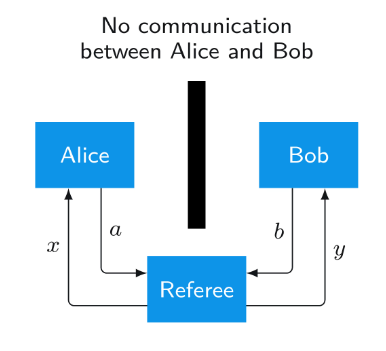
\includegraphics[width=0.5\linewidth]{Images/chsh.png}
\end{figure}

it is the uncertainty about which questions will be asked, and specifically the fact that each player doesn't know the other player's question, that makes non local games challenging for Alice and Bob - just like colluding suspects in different rooms trying to keep their story straight.

A precise description of the referee defines an instance of a nonlocal game. This includes a specification of the probabilities $p(x,y)$ for each question pair along with the rules that determine whether a pair of answers $(a,b)$ wins or loses for each possible question pair $(x,y)$.

We'll take a look at the CHSH game momentarily, but it's also interesting to consider other non local games. Some non local games are fascinating and mysterious to this day, and some aren't so interesting. While the set-up is simple, there's complexity at work - and for some nonlocal games it can be impossibly difficult to compute best or near best strategies for Alice and Bob. This is part of the fascinating nature of the non-local games model.

\subsubsection{CHSH game description}
Here is the precise description of the CHSH game, where (as above) $x$ is Alice's question, $y$ is Bob's question, $a$ is Alice's answer, and $b$ is Bob's answer:
\begin{enumerate}
    \item The questions and answers are all bits: $x,y,a,b \in \{0,1\}$.
    \item The referee chooses the questions $(x,y)$ uniformly at random. That is, each of the four possibilities. $(0,0),(0,1),(1,0),(1,1)$ is selected with probability $1/4$.
    \item The answers $(a,b)$ win for the questions $(x,y)$ is $a \oplus b= x \land y$ and lose otherwise. The following table expresses this rule by listing the winning and losing conditions on the answers ($a,b$) for each pair of questions $(x,y)$.
    
    \begin{table}[ht]
        \centering
        \begin{tabular}{|c|c|c|}
        \hline
             $(x,y)$ & win  & lose \\
             \hline
             $(0,0)$ & $a=b$ & $a \neq b$\\
             \hline
             $(0,1)$ & $a=b$ & $a \neq b$\\
             \hline
             $(1,0)$ & $a=b$  & $a \neq b$\\
             \hline
             $(1,1)$ & $a\neq b$ & $a=b$ \\
             \hline
        \end{tabular}
        \caption{Winning and losing answers $(a,b)$ for each pair of questions $(x,y)$ in the CHSH game}
        \label{tab:chsh_win_lose}
    \end{table}
\end{enumerate}

\subsubsection{Limitations of classical strategies}
Now let's consider strategies for Alice and Bob in the CHSH game, beginning with classical strategies.

\subsubsection{Deterministic Strategies}
We'll start with deterministic strategies, where Alice's answer $a$ is a function of the question$x$ that she receives, and likeise Bob's answer $b$ is a function of the question $y$ he receives. So, for instance, we may write $a(0)$ to represent Alice's answer then her question is $0$, and $a(1)$ to represent Alice's answer when her question is $1$.

No deterministic strategy can possibly win the CHSH game every time. One way to response this is simply to go one-by-one through all of the possible deterministic strategies and check that every one of them losses for at least one of the four possible question pairs. Alice and Bob can each choose from four possible question pairs. Alice and bob can each choose from four possible functions from one bit to one bit - which we encountered and so there are 16 different deterministic strategies in total to check.

We can also reason this fact analytically. If Alice and Bob's strategy wins when $(x,y)=(0,0)$, the it must be that $a(0)=b(0)$; if their strategy wins for $(x,y)=(0,1)$, we conclude that $a(0)=b(0)$; if their strategy wins for $(x,y)=(0,1)$, we conclude that $a(0)=b(1)$; and similarly, if the strategy wins for $9x,y)=(1,0)$, then $a(1)=b(0)$. So, if their strategy wins for all three possibilities, then we have
\[
b(1)=a(0)=b(0)=a(1)
\]
This implies that the strategy loses in the final case $(x,y)=(1,1)$, for here winning requires that $a(1) \neq b(1)$.

Thus, there can be no deterministic strategy that wins every time. It's easy to find strategies that win in three of the fours cases (such as $a(0)=a(1)=b(0)=b(1)=0$), and so we see that the maximum probabilities for Alice and Bob to win using a deterministic strategy is $3/4$.

\subsubsection{Probabilistic Strategies}
As we just concluded, Alice and Bob cannot do better than winning the CHSH game $75\%$ of the time using a deterministic strategy. but what about a probabilistic strategy? Could it help Alice and Bob to use randomness - including the possibility of shared randomness, where their random choices are correlated?

It turns out that probabilistic strategies don't help at all to increase the probability that Alice and Bob win. This is because every probabilistic strategy can alternatively be viewed as a random selection of a deterministic strategy, just like probabilistic operations can be viewed as random selections of deterministic operations. The average is never larger than the maximum, and so it follows that probabilistic strategies don't offer any advantage in terms of their overall winning probability.

Thus, winning with probability $3/4$ is the best that Alice and Bob can do using any classical strategy, whether deterministic or probabilistic.

\subsubsection{CHSH game strategy}
A natural question to ask at this point is whether Alice and Bob can do any better using a quantum strategy. In particular, if they share an entangled quantum state as the following figure suggests, can they increase their winning probability?
\begin{figure}[ht]
    \centering
    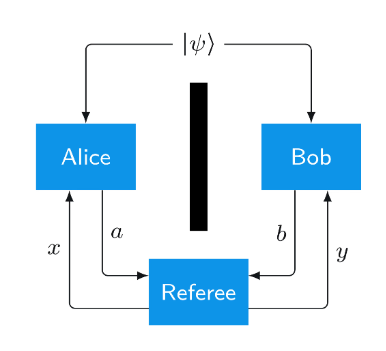
\includegraphics[width=0.5\linewidth]{Images/chsh_game.png}
\end{figure}
The answer is yes, and this is the main point of the example and why it's so interesting. So let's see exactly how alice and Bob can do better in this game using entanglement.

\subsubsection{Required vectors and matrices}
The first thing we need to do is define a qubit state vector $\ket{\psi-{\theta}}$, for each real number $\theta$ (which we'll think of as an angle measured in radians) as follows.
\[
\ket{\psi_{\theta}} = \cos(\theta)\ket{0} + \sin(\theta)\ket{1}
\]
Here are some simple examples:
\begin{align*}
    \ket{\psi_0} &= \ket{0}\\
    \ket{\psi_{\pi/2}}&=\ket{1}\\
    \ket{\psi_{\pi/4}} &=\ket{+}\\
    \ket{\psi_{-\pi/4}} =\ket{-}
\end{align*}
We also have the follwing examples, whic arise in the analysis below:
\begin{align*}
    \ket{\psi_{-\pi/8}} &= \frac{\sqrt{2+\sqrt{2}}}{2}\ket{0}-\frac{\sqrt{2-\sqrt{2}}}{2}\ket{1}\\
    \ket{\psi_{\pi/8}} &= \frac{\sqrt{2+\sqrt{2}}}{2}\ket{0}+\frac{\sqrt{2-\sqrt{2}}}{2}\ket{1}\\
    \ket{\psi-{3\pi/8}} &=\frac{\sqrt{2-\sqrt{2}}}{2}\ket{0} + \frac{\sqrt{2+\sqrt{2}}}{2}\ket{1}\\
    \ket{\psi_{5\pi/8}} &= -\frac{\sqrt{2-\sqrt{2}}}{2}\ket{0} + \frac{\sqrt{2+\sqrt{2}}}{2} \ket{1}
\end{align*}
Looking at the general form, we see that the inner product between any two of these vectors has this formula:
\[
\braket{\psi_{\alpha}|\psi_{\beta}} =\cos(\alpha) \cos(\beta) + \sin(\alpha)\sin(\beta) = \cos(\alpha-\beta)
\]
In detail, we only have real number entries in these vectors, so there are no complex conjugates to worry about: the inner product is the product of the cosines plus the product of the sines. We can then use one of the so-called angle addition formulas to simplify. This formula reveals the geometric interpretation of the inner product between real unit vectors, as the cosine of the angle between them.

Now, if we compute the inner product of the tensor product of any two of these vectors with the $\ket{\phi^+}$ state we obtain a similar expression, except that it has a $\sqrt{2}$ in the denominator.

\section{Implementation using Qiskit}
\textbf{Background}\\
Usage estimate: 4 seconds on ibm\_kyoto (NOTE; This is an estimate only. Your runtime may
vary)

In order to run the superdense coding circuit as shown in figure \ref{fig:superdense-coding}, we are require to program an oracle which will implement the required gates based on the classical bit inputs given by Alice to be transmitted to Bob.\\
\textbf{Requirements}\\
Before starting this tutorial, ensure that you have the following installed:
\begin{itemize}
\item Qiskit SDK 1.0 or later, with visualization support (pip install 'qiskit[visualization]')
\item Qiskit Runtime (pip install qiskit-ibm-runtime) 0.22 or later
\end{itemize}
\textbf{Setup}\\
Here we import the small number of tools we need for this tutorial
\begin{lstlisting}[language=Python]
#Built-in modules
import math

#imports from Qiskit
from qiskit import QuantumCircuit, QuantumRegister, ClassicalRegister
from qiskit.visualization import plot_distribution

#Imports from Qiskit Runtime
from qiskit_ibm_runtime import QiskitRuntimeService
from qiskit_ibm_runtime import SamplerV2 as Sampler
\end{lstlisting}
\begin{lstlisting}[language=Python]
# To run on hardware, selectthe backedn with the fewest number of jobs in the queue
service = QiskitRuntimeService(channel="ibm_quantum")
backend = service.least_busy(operational=True, simulator=False)
backend.name
\end{lstlisting}
This outputs one of the IBM hardware (say ibm\_kyoto).
\begin{enumerate}
    \item \textbf{Step 1: Map classical inputs to a quantum problem}: \\
   In order to implement an oracle which maps the classical inputs to a quantum problem of superdense coding we use qiskit circuit library to setup a 2-qubit oracle which implements the required gates based on the classical bits as given in figure \ref{fig:superdense2}. The runtime sampler is used for execution of the circuit.
   
\begin{lstlisting}[language=Python]
def superdense_circuit(string):
    # Create a Quantum Circuit
    qubits=QuantumRegister(2,name="q")
    cbits=ClassicalRegister(2,name="c")
    circuit = QuantumCircuit(qubits,cbits)
    
    q0,q1=qubits
    c0,c1=cbits

    # Prepare the state to be teleported
    circuit.h(q0)
    circuit.cx(q0, q1)

    circuit.barrier()

    if string[0]=="1":
        circuit.z(q0)
    if string[1]=="1":
        circuit.x(q0)

    circuit.barrier()
    
    circuit.cx(q0, q1)
    circuit.h(q0)

    circuit.barrier()
    
    circuit.measure(q0, c0)
    circuit.measure(q1, c1)

    return circuit    
    \end{lstlisting}
    Note that the above code implements the oracle based on the input given. It can be seen that it clearly implements the oracle according to the Alice's encoding based on the classical bits she wishes to transmit to Bob according to the figure \ref{fig:superdense2}.
    \begin{lstlisting}[language=Python]
qc_00=superdense_circuit("00")
qc_01=superdense_circuit("01")
qc_10=superdense_circuit("10")
qc_11=superdense_circuit("11")
    \end{lstlisting}
    The above code will create quantum circuits which will encode Alice's classical bits to be transmitted to Bob into the circuit using the oracle.
    \begin{lstlisting}[language=Python]
qc_00.draw('mpl')
    \end{lstlisting}
    Similarly any other circuit can be created by changing the syntax parameters.
    The circuit along with the corresponding oracle implementing the function is as shown in the figure \ref{fig:superdense_circuit}.
     \begin{figure}[ht]
        \centering
        \begin{subfigure}[b]{0.45\linewidth}
        \centering
        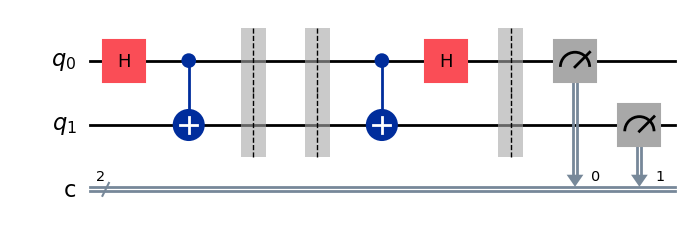
\includegraphics[width=1\linewidth]{Images/superdense_00.png}
        \caption{Classical bits: 00}
        \label{fig:superdense_00}
        \end{subfigure}
        \hfill
        \centering
        \begin{subfigure}[b]{0.45\linewidth}
        \centering
        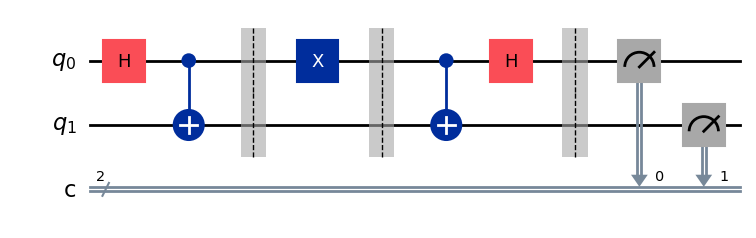
\includegraphics[width=1\linewidth]{Images/superdense_01.png}
        \caption{Classical bits: 01}
        \label{fig:superdense_01}
        \end{subfigure}
        \vspace{0.5 cm}
        \begin{subfigure}[b]{0.45\linewidth}
        \centering
        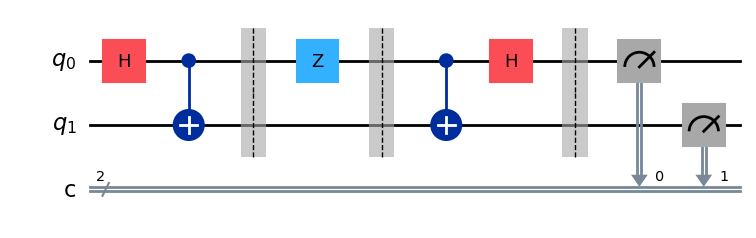
\includegraphics[width=1\linewidth]{Images/superdense_10.png}
        \caption{Classical bits: 10}
        \label{fig:superdense_10}
        \end{subfigure}
        \hfill
        \begin{subfigure}[b]{0.45\textwidth}
        \centering
        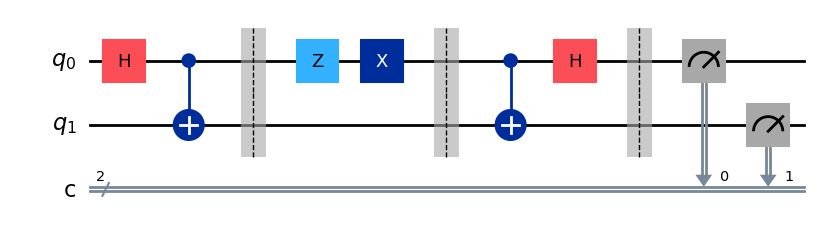
\includegraphics[width=1\linewidth]{Images/superdense_11.png}
        \caption{Classical bits: $11$}
        \label{fig:superdense_11}
        \end{subfigure}    
        \caption{Superdense Coding Circuits based on the classical bits Alice wishes to transmit to Bob}
        \label{fig:superdense_circuit}
    \end{figure}
    Note that the oracle (shown between the two barriers) implements the required gates corresponding to the classical bits. Thus the above shown figure corresponds to the Superdense coding circuit.
    \item \textbf{Step 2: Optimize Problems for Quantum Execution}
\begin{lstlisting}[language=Python]
from qiskit.transpiler.preset_passmanagers import generate_preset_pass_manager

target=backend.target
pm = generate_preset_pass_manager(backend=backend, optimization_level=3)

circuit_isa_00=pm.run(qc_00)
circuit_isa_00.draw(output="mpl",idle_wires=False,style="iqp")\end{lstlisting}

\begin{figure}[ht]
        \centering
        \begin{subfigure}[b]{0.45\linewidth}
        \centering
        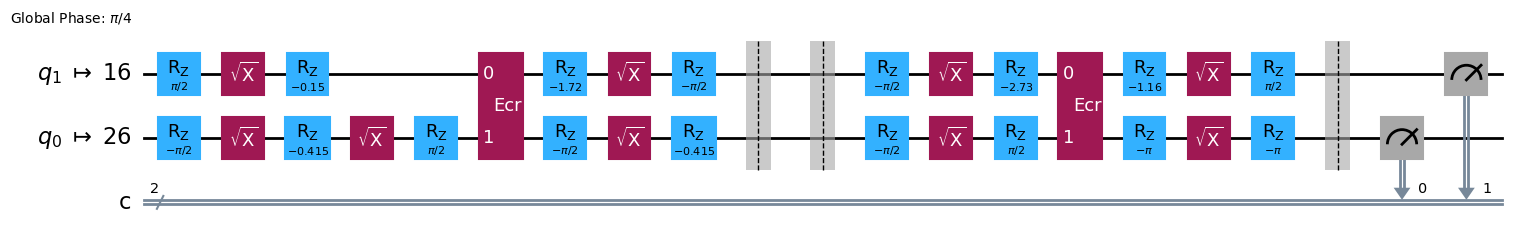
\includegraphics[width=1\linewidth]{Images/opt_superdense_00.png}
        \caption{Classical bits: 00}
        \label{fig:opt_superdense_00}
        \end{subfigure}
        \hfill
        \centering
        \begin{subfigure}[b]{0.45\linewidth}
        \centering
        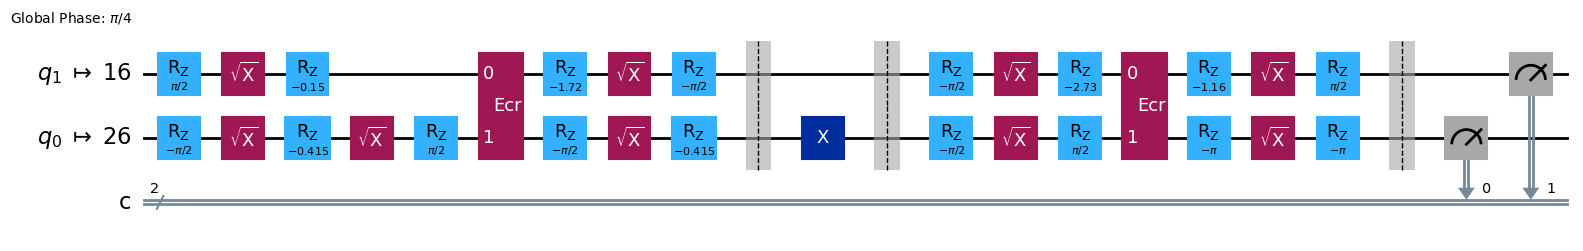
\includegraphics[width=1\linewidth]{Images/opt_superdense_01.png}
        \caption{Classical bits: 01)}
        \label{fig:opt_superdense_01}
        \end{subfigure}
        \vspace{0.5 cm}
        \begin{subfigure}[b]{0.45\linewidth}
        \centering
        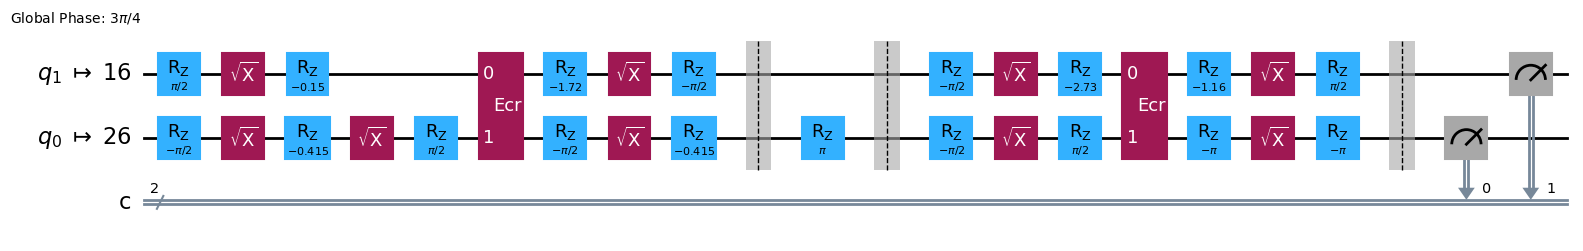
\includegraphics[width=1\linewidth]{Images/opt_superdense_10.png}
        \caption{Classical bits: 10}
        \label{fig:opt_superdense_10}
        \end{subfigure}
        \hfill
        \begin{subfigure}[b]{0.45\textwidth}
        \centering
        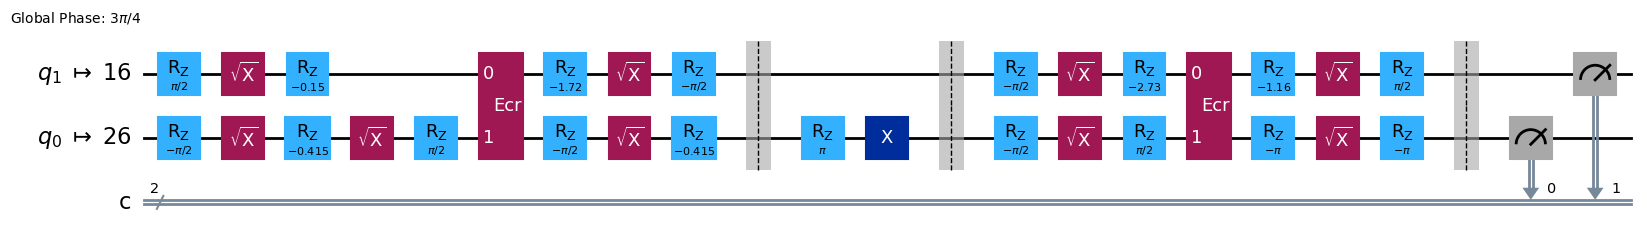
\includegraphics[width=1\linewidth]{Images/opt_superdense_11.png}
        \caption{Classical bits: 11}
        \label{fig:opt_superdense_11}
        \end{subfigure}    
        \caption{Optimized Superdense coding Circuit implementation for transmitting possible classical bits along with their corresponding oracles}
        \label{fig:superdense_opt_circuit}
    \end{figure}
    The Optimized circuit shown in figure \ref{fig:superdense_opt_circuit} are the ones that actually get executed on a quantum computer as they are optimized for the target hardware.
    \item \textbf{Step 3: Execute using Qiskit Primitives}\\
    We are now required to run the circuit and sample the measurements on the two qubits. Thus for execution we will use the Sampler runtime primitive.
    \begin{lstlisting}[language=Python]
# TO run on local simulator:
#1. Use the StatevectorSampler from qiskit.primitves instead
sampler=Sampler(backend=backend)
sampler.options.default_shots=10_000
result_00 = sampler.run([circuit_isa_00]).result()
dist_00 = result_00[0].data.c.get_counts()  
    \end{lstlisting}
    The output of the above code will be the distribution of the measurements on the two qubits. Similar code can be written for all the other circuits by just implementing the required oracle.

    \item \textbf{Step 4: Post-Process Results}\\
    Now we plot a histogram of the measurements on the two qubits in the classical format.
    \begin{lstlisting}[language=Python]
from qiskit.visualization import plot_histogram
plot_histogram(dist_00)
    \end{lstlisting}
    The output of the above code will be the histogram of the distribution of the measurements on the first two qubits. Similar code can be written for all the other possible classical bits.

    The following output is produced upon running this code on ibm\_brisbane as shown in figure \ref{fig:deutsch_jozsa_results}. The histogram plot is done for 10000 shots and results can be clearly seen as expected. The minor deviations in the results is due to the inherent errors (because of the noise) in the quantum computer and its probabilistic nature in the measurement process.
    \begin{figure}
        \centering
        \begin{subfigure}[b]{0.45\linewidth}
        \centering
        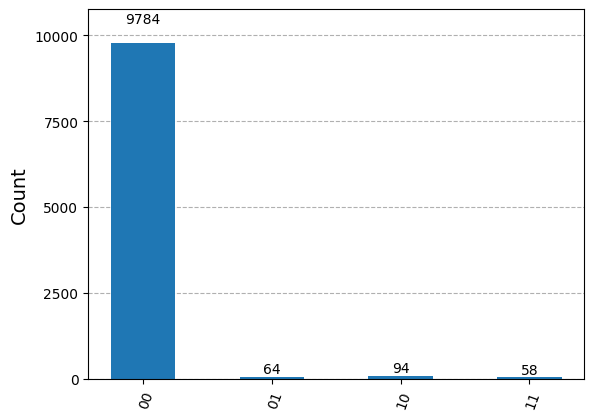
\includegraphics[width=1\linewidth]{Images/results_superdense_00.png}
        \caption{Classical bits: 00}
        \label{fig:results_superdense_00}
        \end{subfigure}
        \hfill
        \centering
        \begin{subfigure}[b]{0.45\linewidth}
        \centering
        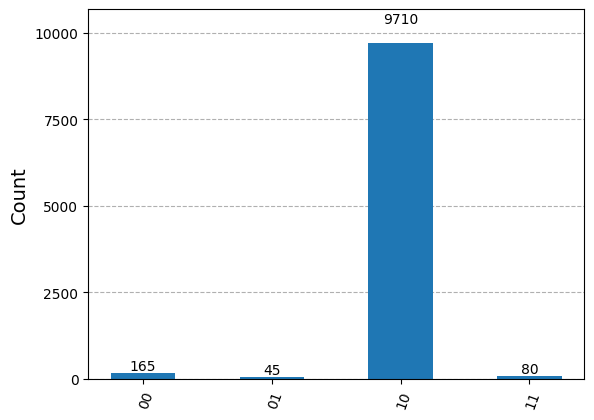
\includegraphics[width=1\linewidth]{Images/results_superdense_01.png}
        \caption{Classical bits: 01}
        \label{fig:results_superdense_01}
        \end{subfigure}
        \vspace{0.5 cm}
        \begin{subfigure}[b]{0.45\linewidth}
        \centering
        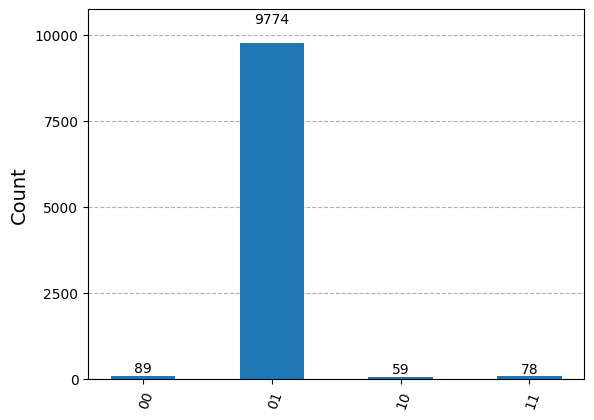
\includegraphics[width=1\linewidth]{Images/results_superdense_10.png}
        \caption{Classical bits: 10}
        \label{fig:rsults_superdense_10}
        \end{subfigure}
        \hfill
        \begin{subfigure}[b]{0.45\textwidth}
        \centering
        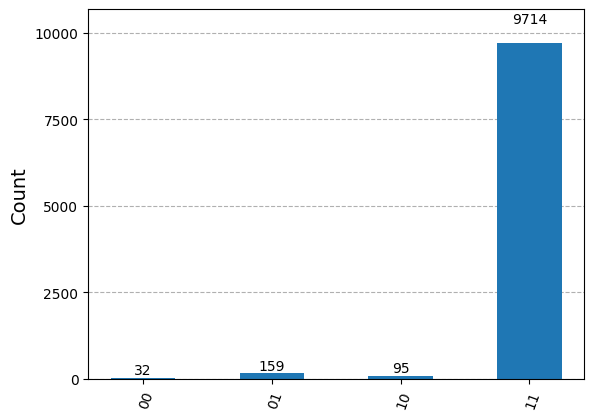
\includegraphics[width=1\linewidth]{Images/results_superdense_11.png}
        \caption{Classical bits: 11}
        \label{fig:results_superdense_11}
        \end{subfigure}    
        \caption{Superdense coding Results}
        \label{fig:superdense_results}
    \end{figure}
    Note in the figure you might see that the results for 01 and 10 are interchanged and one might think this as a mistake but it is not. Qiskit uses little-endian both for classical bit and qubit ordering. So the classical bits are read from right to left. Thus, the results.
\end{enumerate}



\chapterreferences
